\documentclass{article}

\usepackage{arxiv}

\usepackage[utf8]{inputenc} % allow utf-8 input
\usepackage[T1]{fontenc}    % use 8-bit T1 fonts
\usepackage[hidelinks]{hyperref}       % hyperlinks
\usepackage{url}            % simple URL typesetting
\usepackage{booktabs}       % professional-quality tables
\usepackage{amsmath,amssymb,amsthm}
\usepackage{amsfonts}       % blackboard math symbols
\usepackage{float}
\usepackage{nicefrac}       % compact symbols for 1/2, etc.
\usepackage{microtype}      % microtypography
\usepackage{mathrsfs}
\usepackage{onimage}
\usepackage{graphicx}
\usepackage{doi}
\usepackage{acronym}
\usepackage{listings}
\usepackage{tikz}
\usepackage{tabularx}
\usepackage{siunitx}
\usepackage{cite}
\usepackage{acronym}
\usepackage{xcolor}

\usetikzlibrary{trees}
\usetikzlibrary{shapes.geometric, arrows}

\definecolor{color1}{HTML}{6bd2db}
\definecolor{color2}{HTML}{0ea7b5}
\definecolor{color3}{HTML}{0c457d}
\definecolor{color4}{HTML}{ffbe4f}
\definecolor{color5}{HTML}{e8702a}

\title{Methods for Analyzing Models of Rod-Shaped Bacteria}

%\date{September 9, 1985}	% Here you can change the date presented in the paper title
%\date{} 					% Or removing it

\author{
    \href{https://orcid.org/0009-0001-0613-7978}{
        
\includegraphics[scale=0.06]{orcid.pdf}
        \hspace{1mm}Jonas Pleyer
    }
    \thanks{
        \href{https://jonas.pleyer.org}{jonas.pleyer.org},
        \href{https://cellular-raza.com}{cellular-raza.com}
    }\\
	Freiburg Center for Data-Analysis and Modeling\\
	University of Freiburg\\
	\texttt{jonas.pleyer@fdm.uni-freiburg.de} \\
	%% examples of more authors
	\And
	\href{https://orcid.org/0000-0002-6371-4495}{
        
\includegraphics[scale=0.06]{orcid.pdf}
        \hspace{1mm}Christian Fleck
    }\\
	Freiburg Center for Data-Analysis and Modeling\\
	University of Freiburg
}

\newacro{abm}[ABM]{Agent-Based Model}
\newacro{ode}[ODE]{Ordinary Differential Equation}
\newacro{pbr}[PBR]{Physically-Based Rendering}

% Uncomment to remove the date
%\date{}

% Uncomment to override  the `A preprint' in the header
\renewcommand{\headeright}{Preprint}
%\renewcommand{\undertitle}{Technical Report}
\renewcommand{\shorttitle}{Methods for Analyzing Models of Rod-Shaped Bacteria}

\usepackage{enumitem}
\setlist{nolistsep}

%%% Add PDF metadata to help others organize their library
%%% Once the PDF is generated, you can check the metadata with
%%% $ pdfinfo template.pdf
\hypersetup{
pdftitle={% TODO
},
pdfsubject={q-bio.NC, q-bio.QM},
pdfauthor={Jonas Pleyer, Christian Fleck},
pdfkeywords={},
}

% Change numbering of equations
% \numberwithin{equation}{section}

% MAKE TITLES IN THEOREMS BOLD
\makeatletter
\def\th@plain{%
  \thm@notefont{}% same as heading font
  \itshape % body font
}
\def\th@definition{%
  \thm@notefont{}% same as heading font
  \normalfont % body font
}
\makeatother

\begin{document}
\maketitle

%###################################################################################################
\begin{abstract}
    This paper establishes the basis for a novel individual-based mechanical model of rod-shaped
    bacteria.
    It describes methods of how to obtain data from microscopic images such that they can be used
    for parameter estimation purposes.
    Furthermore, we show initial results for parameter estimates and an application of the model to
    the formation of multilayers within bacterial colonies.
\end{abstract}

% keywords can be removed
% \keywords{}

\tableofcontents

%###################################################################################################
\section{Introduction}
\label{section:introduction}

Bacteria exist in many physical shapes such as spheroidal, rod-shaped or spiral
\cite{Zapun2008,Young2006}.
The last decades have fundamentally challenged and changed our understanding of how bacteria retain
their shape.
Rod-shaped bacteria can grow by extending their circular part, or by inserting new material at the
tip of the rod.
Species such as E.coli and B.subtilis~\cite{Errington2020} fall under the first category while
S.pombe represents the latter.
New material is inserted in small bursts on the nanoscale in forms of patches, bands or
hoops~\cite{DePedro2003}.
Despite their differences in wall-size, B.subtilis and E.coli follow growth rules which are
comparable with respect to the extension of the rod~\cite{Chang2014}.

\begin{itemize}
    \item This publication contains 5 things:
    \begin{enumerate}
        \item Methods of how to obtain data from microscopic images and perform parameter
            estimations; $\rightarrow$ also possibly across multiple generations
        \item Showcase the usefulness of the methods and the model by applying it to parameter
            estimation via microscopic images and multilayer formation
        \item Initial (incomplete) model of rod-shaped bacteria
        \item Generate 3D Images (masks)
        \item A python package which can do all of that and can be reused and extended
    \end{enumerate}
    \item Overall structure
    \begin{enumerate}
        \item users bring model + data
        \item this paper provides methods to do the parameter estimation + visualization
    \end{enumerate}
    \item For complete model, more work has to be done
    \begin{itemize}
        \item More aspects (see Review; put in discussion)
        \item Note that we only care about \textit{E.Coli} and \textit{B.Subtilits}! This is
            important.
    \end{itemize}
\end{itemize}

\begin{figure}[H]
    \centering
    \tikzstyle{rect} = [
        rectangle,
        % rounded corners,
        minimum width=4cm,
        minimum height=1cm,
        text centered,
        draw=black,
        fill=color4!70,
    ]
    \tikzstyle{brect} = [rect, fill=color5!50]
    \tikzstyle{frect} = [rect, fill=color3!40]
    \tikzstyle{arrow} = [thick,->,>=stealth]
    \tikzstyle{darrow} = [arrow, dashed]
    \begin{tikzpicture}
        \node (model) [brect, align=center] at (0,0) {Mathematical \&\\ Computational Model};
        \node (extraction) [rect] at (0, -2) {Data Extraction};
        \node (params) [brect] at (6, -2) {Parameter Estimation};
        \node (visualization) [rect] at (6, 0) {Visualization};

        \draw[arrow] (model) -- (extraction);
        \draw[darrow] (params) -- node[anchor=south, rotate=-18.43] {validate} (model);
        \draw[arrow] (model) -- (visualization);
        \draw[arrow] (visualization) -- (params);
        \draw[arrow] (extraction) -- (params);

        % Future stuff
        \node (realimages) [frect] at (12, 0) {Data Generation};
        \node (segmentation) [frect] at (12, -2) {Cell Segmentation};
        \node (tracking) [frect] at (12, -3) {Cell Tracking};
        \node (analysis) [frect] at (0, -4) {Analysis Methods};

        \draw[arrow] (visualization) -- (realimages);
        \draw[arrow] (realimages) -- (segmentation);
        \draw[arrow] (extraction) -- (analysis);
        \draw[arrow] (params) -- (realimages);
    \end{tikzpicture}
    \caption{
        The project can be divided into 4 subparts (orange + yellow) that interact with and depend
        on each other.
        The orange blocks require input by the user by specifying the model and supplying input
        data.
        Additional blocks (blue-gray) indicate possible future extensions of this project.
        Arrows with solid lines indicate dependencies between the subparts while dashed arrows carry
        special meaning, which is specifically annotated.
        The mathematical models provides the theoretical framework and is thus the parent of all
        following work.
        "Data Extraction" allows us to read variable and parameter values directly from microscopic
        images.
        The obtained data can then be used to initialize a numerical simulations and thus estimate
        parameters.
        On the other hand, results produced by our model can be visualized as 3D renders and
        projected to cell-masks.
        These algorithms can be exploited to construct cost-functions which can be used in the
        parameter estimation process.
        In future work, this visualization scheme could be extended to generate realistic
        microscopic images with cell-masks and thus train cell-segmentation and cell-tracking
        algorithms.
    }
    \label{fig:flowchart-project-structure}
\end{figure}

% TODO write more text here
% Use some parts of the proposal text

%###################################################################################################
\section{Fundamental Assumptions on the Spatial Representation of Rod-Shaped Bacteria}
% TODO CITATIONS
This work makes use of a few but powerfull assumptions concerning the mathematical representation of
the cells in question.
In order to describe the spatial dynamics of individual agents, we need to define their position,
shape and how they interact with each other.
In order to provide as much flexibility as possible when constructing new models, we restrict
ourselves to assumptions concerning the position such that researchers can freely experiment with
various shapes and interaction types.
Furthermore, it is very important to strike a good balance between the restrictiveness of our
assumptions and generality in order to provide meaningful results and still be able to apply our
approach to a broader class of models.
Taking into account the natural shape of rod-like bacteria, it is clear that they can not be
represented with a singular point $\vec{v}$ in space.
We could extend this positional definition with a vector $\vec{w}$, indicating the direction of
extension but this would restrict ourselves to fully straight rod-shaped bacteria.
However, multiple experiments have shown that MReB is responsible for the growth and maintenance of
the elongated shape of bacteria~\cite{Erickson2001}.
By means of this protein, rod-shaped bacteria can bend elastically on short time-scales and
deform plastically over longer periods of time.
Our goal is to provide a model which can encapsulate these effects.
Thus, we extend our model from a single point to multiple vertices which are part of a 1-dimensional
polygon with two endpoints $\vec{v}_i$.
In essence, we discretize the (possibly non-straight) rod of the agent.
Figure~\ref{fig:mechanics-bacterium} shows a visualization of this approach.
The angles $\alpha_i$ between vertices $\vec{v}_{i-1},\vec{v}_i$ can be used when modeling the
dynamics of these bacteria.

With these fundamental thoughts layed out, we retain the flexibility to represent many models such
as varying shapes since we do not have to make any assumptions on the type of interactions between
two bacteria.
Even concerning the shape of bacteria, this assumption still allows us to mdoel elliptical cells by
modifying the interaction type as well as other effects such as polarity of
interactions~\cite{Duvernoy2018}.
Furthermore, we also did not have to assume any particular mechanical dynamics of the agents, only
their spatial representation, thus leaving in particular room for plastical or elastic deformations
of the rod and other more intricate mechanisms.

\begin{enumerate}
    \item represent bacteria as polygon with vertices $\vec{v}_i$
    \item Assumes that these vertices are not fundamental but rather a discretization of the actual
        problem
\end{enumerate}

\begin{figure}[H]
    \centering
    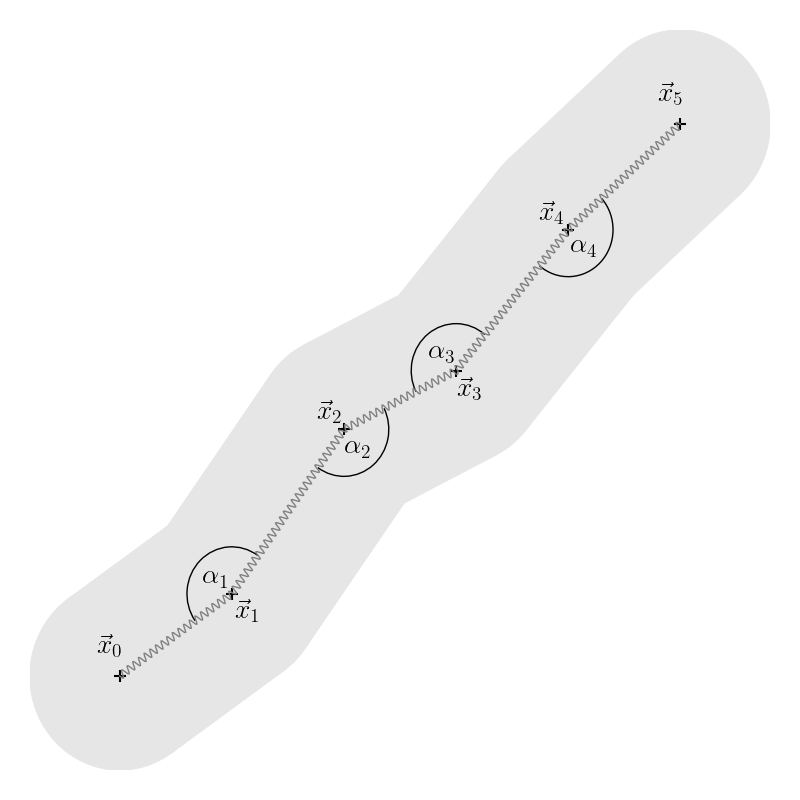
\includegraphics[width=0.5\textwidth]{docs/source/_static/mechanics.png}
    \caption{
        Example of an elonged bacterial rod represented by a collection of vertices which are
        connected by springs.
        The angles $\alpha_i$ have been exaggerated such that they can be identified more easily.
        A bacterial agent which is not interacting with any external objects will tend to the
        equilibrium state of a straight rod with $0$ curvature.
    }
    \label{fig:mechanics-bacterium}
\end{figure}

%###################################################################################################
\section{Data Extraction}
\label{section:fitting-and-comparing-masks}

This section will explain how we can determine the collection of vertices $\vec{v}_i$ introduced in
subsection~\ref{subsection:mechanical-model-mechanics} from microscopic images
(Figure~\ref{fig:position-extraction-algorithm} (A)).
They will serve as initial, final and intermediate values with which we can compare our predictions.
The algorithms which we devised requires the input of cell-masks which assign a unique color for
every cell in the image.
Such masks can be generated by cell-segmentation tools or obtained by annottating microscopic images
by hand (Figure~\ref{fig:position-extraction-algorithm} (B)).
Afterwards, we proceed with the following 5 steps.
\begin{enumerate}
    \item Obtain submasks for each cell individually.
    \item Skeletonize submask with algorithm from Lee~\cite{Lee1994}
    \item Determine endpoints $\vec{q}_0,\vec{q}_1$.
        Assert that there are only 2 endpoints.
    \item Sort points such that they form a polygon.
    \item Interpolate vertices $\vec{v}_i$ from obtained polygon.
\end{enumerate}
In the first step, the image will be split into a collection of subimages that only contain
information for one single cell.
From there, we apply a skeletonization algorithm~\cite{Lee1994}
(Figure~\ref{fig:position-extraction-algorithm} (C)).
It has to be noted that there are multiple variants of skeletonization and in general, these classes
of algorithms can produce results which have intersection points and multiple endpoints.
This described behaviour is undesirable in our case.
We have found that for most practical examples, the algorithm devised by~\cite{Lee1994} has worked
well.\\
The skeletonization algorithm supplies us with a collection of unordered lattice points $\vec{p}_i$
(pixel coordinates) where the skeleton lives.
We identify the endpoints $\vec{q}_0,\vec{q}_1$ by counting the number of neighbors in the von
Neumann neighborhood for each lattice point.
Any point with exactly one neighboring point must be and endpoint.
If we encounter more or less than two points which fit this criterion, the routine can not commence
and is aborted.
Next, we start with one of the endpoints and determine the next neighbor which was not yet picked.
We list the points in this order, thus forming a sorted polygon of pixel coordinates.\\
In the last step, we take the sorted, extracted points $\vec{p}_i$ and interpolate $n$ values for
the desired number of vertices $\vec{v}_i$.

\begin{figure}
    \centering
    \begin{tikzonimage}[width=0.32\textwidth]
        {docs/source/_static/fitting-methods/algorithm/image001042.png}
        \node at (0.025, 0.975)[anchor=north west, rectangle, draw, white, minimum width=15pt, minimum height=15pt]{\textbf{A}};
    \end{tikzonimage}
    \begin{tikzonimage}[width=0.32\textwidth]
        {docs/source/_static/fitting-methods/algorithm/mask-zoom.png}
        \node at (0.025, 0.975)[anchor=north west, rectangle, draw, white, minimum width=15pt, minimum height=15pt]{\textbf{B}};
    \end{tikzonimage}
    \begin{tikzonimage}[width=0.32\textwidth]
        {docs/source/_static/fitting-methods/algorithm/mask-zoom.png}
        \node at (0.025, 0.975)[anchor=north west, rectangle, draw, white, minimum width=15pt, minimum height=15pt]{\textbf{C}};
    \end{tikzonimage}
    \caption{
        TODO change 2nd image!\\
        (A) An example of a microscopic image.
        (B) The associated mask which assigns individual color values to each bacterium.
        (C) The result of the  skeletonization algorithm when applying it to a single cell.
    }
    \label{fig:position-extraction-algorithm}
\end{figure}

% --------------------------------------------------------------------------------------------------
\paragraph{Benchmarking the Extraction Algorithm}
\label{subsection:benchmarking-extraction-algorithm}

In order to determine if our extraction algorithm provides reliable results, we have to take
advantage of a functionality which will be introduced later in
section~\ref{section:generating-masks-and-images}.
Our methodology makes use of the fact that we have already set up our model and solving scheme and
are able to produce cell masks from these numerical results.
In doing so, we have exact knowledge about the position of our agents since we can simply obtain
this information from our model.
But on the other hand we can also try to extract this position from the generated cell-masks.
By comparing the differences between them, we get a good estimate of how well our extraction
algorithm can determine the true position of the bacteria.

In figure~\ref{fig:benchmarking-extraction-algorithm} (A-C) we see snapshots of a time series of
masks.
This particular simulation includes division events between images (B) and (C).
For all images (A-C), we have drawn the exact position of the agents with white lines and indicated
the extracted positions with crosses.
They align very well visually.
It may be hard to spot with the bare eye, but the agreement between extracted and exact positions is
visually worse at the endpoints of the rods.
To quantify this disparity, we calculate the distance between these individual vertices.
Figure~\ref{fig:benchmarking-extraction-algorithm} (D) shows the estimated length of the rods from
the extracted and exact vertices which is surrounded by the average vertex distance.
Division events lead to steps in our rod-length function since the bacterial length is halved.
We can clearly see that the agreement is very good in the beginning but right after every division
event, the uncertainty becomes large.
To illustrate this, we can see that in figure~\ref{fig:benchmarking-extraction-algorithm} (C) some
of the rods are partially overlapping which hides parts of the individual cell-masks and thus
changes the extraction result.
We also plotted the distribution of individual vertex distances in
figure~\ref{fig:benchmarking-extraction-algorithm} (E).
Darker areas in the plot correspond to distances at time-points earlier in the simulatin time.
We can see that brighter areas tend to shift towards the right, thus increasing the uncertainty of
the extraction.
However, the overall distribution shows small values of distances for a large number of vertices and
is not dominated by outliers.

\begin{figure}
    \centering
    \begin{tikzonimage}[width=0.32\textwidth]
        {docs/source/_static/fitting-methods/extract_positions-004000.png}
        \node at (0.025, 0.975)[anchor=north west, rectangle, draw, white, minimum width=15pt, minimum height=15pt]{\textbf{A}};
    \end{tikzonimage}
    \begin{tikzonimage}[width=0.32\textwidth]
        {docs/source/_static/fitting-methods/extract_positions-006000.png}
        \node at (0.025, 0.975)[anchor=north west, rectangle, draw, white, minimum width=15pt, minimum height=15pt]{\textbf{B}};
    \end{tikzonimage}
    \begin{tikzonimage}[width=0.32\textwidth]
        {docs/source/_static/fitting-methods/extract_positions-008000.png}
        \node at (0.025, 0.975)[anchor=north west, rectangle, draw, white, minimum width=15pt, minimum height=15pt]{\textbf{C}};
    \end{tikzonimage}
    \begin{tikzonimage}[width=0.5\textwidth]
        {docs/source/_static/fitting-methods/displacement-calculations.png}%
        \node at (0.03, 0.99)[anchor=north west, rectangle, draw, black, minimum width=15pt, minimum height=15pt]{\textbf{D}};
    \end{tikzonimage}%
    \begin{tikzonimage}[width=0.5\textwidth]
        {docs/source/_static/fitting-methods/displacement-distribution.png}
        \node at (0.03, 0.99)[anchor=north west, rectangle, draw, black, minimum width=15pt, minimum height=15pt]{\textbf{E}};
    \end{tikzonimage}
    \caption{
        Progression of generated masks with estimated and exact positions.
        Comparison of masks across generations. Compare estimated with exact rod lengths.
    }
    \label{fig:benchmarking-extraction-algorithm}
\end{figure}


%###################################################################################################
\section{Visualization}
\label{section:generating-masks-and-images}
\begin{itemize}
    \item use pyvista (VTK) for Visualization
    \item always do 3D render. This way, we can have overalp between agents and produce more
        realistic masks.
    \item Assign unique color values for idividual agents.
        We have a 1:1 mapping between agent identifier and color! (for each simulation different
        though)
    \item use parallel projection; this should be most close to what microscopes measure due to the
        relatively large distance between object and lens.
    \item use some noise to smear out the rods; this is already similar to microscopic images; use
        more like this and deal with real-world defects to make it more realistic (future, not now)
    \item Figure~\ref{fig:progression-image-generation} shows steps in generating image.
    \item Reflectivity, placement of light etc. can already introduce some heterogeneity in the
        visual of the rod.
    \item Plan to implement noise on the mesh itself; make it have rough surface (like real rods as
        seen under electron microscopy)
\end{itemize}

\paragraph{Algorithm}
\begin{enumerate}
    \item Get position of cell
    \item Insert spheres at each vertex
    \item Insert cylinder along edges
    \item Combine individual objects into one big mesh
    \item Use \ac{pbr}
\end{enumerate}

\begin{figure}[H]
    \centering
    \begin{tikzonimage}[width=0.3\textwidth]
        {docs/source/_static/09395645494836445480/raw_pv/000000400.png}
        \node at (0.025, 0.975)[anchor=north west, rectangle, draw, white, minimum width=15pt, minimum height=15pt]{\textbf{A}};
    \end{tikzonimage}
    \begin{tikzonimage}[width=0.3\textwidth]
        {docs/source/_static/09395645494836445480/images/000000400.png}
        \node at (0.025, 0.975)[anchor=north west, rectangle, draw, white, minimum width=15pt, minimum height=15pt]{\textbf{B}};
    \end{tikzonimage}
    \begin{tikzonimage}[width=0.3\textwidth]
        {docs/source/_static/09395645494836445480/masks/000000400.png}
        \node at (0.025, 0.975)[anchor=north west, rectangle, draw, white, minimum width=15pt, minimum height=15pt]{\textbf{C}};
    \end{tikzonimage}
    \caption{
        (A) shows the raw result from combining sphere and cylinder meshes to obtain the shape of a
        bacterial rod.
        This render contains lighting coming from 2 light sources which thus produces a small glow
        on the upper part of the meshes.
        Subfigure (B) takes this image and applies noise to it in order to make it look more
        like an actual microscopic image.
        (C) The render is projected along the z-axis and flat numerical values are assigned to the
        bacteria.
        The resuling render can have overlaps in which case the color of the rod is displayed that
        is higher along the z-direction.
    }
    \label{fig:progression-image-generation}
\end{figure}

%###################################################################################################
\section{Parameter Estimation}
In order to effectively estimate the parameters of our model, we need to set up a cost function
which can be minimized.
In doing so, we hope to identify all parameters, given relevant experimental data.
We use microscopic images and construct a novel algorithm that can extract the position of the agent
from a provided cell-mask.
These cell-masks are easily obtainable by either using existing segmentation tools or manually
annottating images.
Following this, we can define a cost-function and an optimization scheme to minimize said function.

% --------------------------------------------------------------------------------------------------
\subsection{Constructing a Loss Function}

As within any optimization scheme, it can be beneficial to construct custom cost functions
which are tailored to the problem at hand.
With the methods that we have already estalished, we need to compare a collection of agents which
were numerically calcualted through our \ac{abm} modeling approach whith microscopic images.
Utilizing the extraction algorithm, we can simply compare the numerically obtained positions with
the extracted positions of the data.
We choose a typical least-squares approach for the comparison of the individual vertices.
However, this procedure is only valid for the case where cell-division events do not play a role.
In the case where we either the numerical model or the experimental data contain more or less cells
than the other result, we are not able to compare them with this approach.

\paragraph{Comparison with Semantic Segmentation}
\label{paragraph:comparison-semantic-segmentation}
\cite{Jadon2020}

\paragraph{Comparison across Generations}
\label{paragraph:comparison-across-generations}

In order to compare a variable amount of cells, we can not utilize the positions of these cells
directly.
In this approach, we propose a method which is similar to already existing routines (TODO mention
machine learning, some vision algorithms use this).
From the numerical results of the \ac{abm}, we can again generate an image of cell-masks.
We then compare this image together to the experimental cell-mask pixel by pixel with each other.
Whenever two pixel colors are not matching, a penalty value is assigned.
The sum of all those penalties is then the total cost.
This algorithm is an implementation of a signed area measure.
It is very important to take into account the parental relationship between the cells, checking if
if either one of the cells is a daughter of the other cell.
If a cell has just divided, the resulting two daughter cells will cover precisely the space that the
preceding agent had taken up.
Let's assume as an example that one result has more cells than the other
(Figure~\ref{fig:mask-difference-metric} (A,B)).
When we compare the pixels of both images, we can relate the given color of the pixel to a certain
cell.
Whenever the colors of two distinct cells are in a parental relationship, we reduce the penalty
which would be assigned or set it to zero.

\begin{figure}
    \centering
    \begin{tikzonimage}[width=0.3\textwidth]
        {docs/source/_static/fitting-methods/progressions-1.png}
        \node at (0.025, 0.975)[anchor=north west, rectangle, draw, white, minimum width=15pt, minimum height=15pt]{\textbf{A}};
    \end{tikzonimage}
    \begin{tikzonimage}[width=0.3\textwidth]
        {docs/source/_static/fitting-methods/progressions-2.png}
        \node at (0.025, 0.975)[anchor=north west, rectangle, draw, white, minimum width=15pt, minimum height=15pt]{\textbf{B}};
    \end{tikzonimage}
    \linebreak
    \begin{tikzonimage}[width=0.3\textwidth]
        {docs/source/_static/fitting-methods/progressions-3.png}
        \node at (0.025, 0.975)[anchor=north west, rectangle, draw, white, minimum width=15pt, minimum height=15pt]{\textbf{C}};
    \end{tikzonimage}
    \begin{tikzonimage}[width=0.3\textwidth]
        {docs/source/_static/fitting-methods/progressions-4.png}
        \node at (0.025, 0.975)[anchor=north west, rectangle, draw, white, minimum width=15pt, minimum height=15pt]{\textbf{D}};
    \end{tikzonimage}
    \caption{
        The figure shows two masks (A,B) which will be compared against each other.
        As we can see, image (B) contains more cells which has resulted from a division process that
        is not yet occurred in image (A).
        In (C) we can see the "naive" comparison, simply identifying non-matching colors.
        By assigning penalties to all highlighted pixels, we would not take into consideration the
        parental relationship.
        This approach is displayed in (D) where pixels of cells that are related have been colored
        in gray.
    }
    \label{fig:mask-difference-metric}
\end{figure}

We can use this procedure to calculate the cost between successive iteration steps
$t_n$ with $t_{n+1}$.
We expect to obtain an exponential growth in the penalty.
This can be explained by to the fact that the growth of the total area is exponential in time.
Furthremore, the temporal area difference can be viewed as a derivative but the derivative of an
exponential is again an exponential.
Figure~\ref{fig:parameter-estimates-single-step} shows the total penalty for this approach.
We can see that by accounting for the parental relationship, we get the overall desired effect.
This method allows us to compare results between states that have a different number of cells
inside as long as their origin stems from the a shared initial state.
However, since this algorithm requires us to calculate a cell-mask for each comparison and then also
process this mask as well as the comparator, it is much more computationally demanding.
In cases where the simpler approach of comparing positions of the agents is reasonable, this method
should be preferred.

\begin{figure}
    \centering
    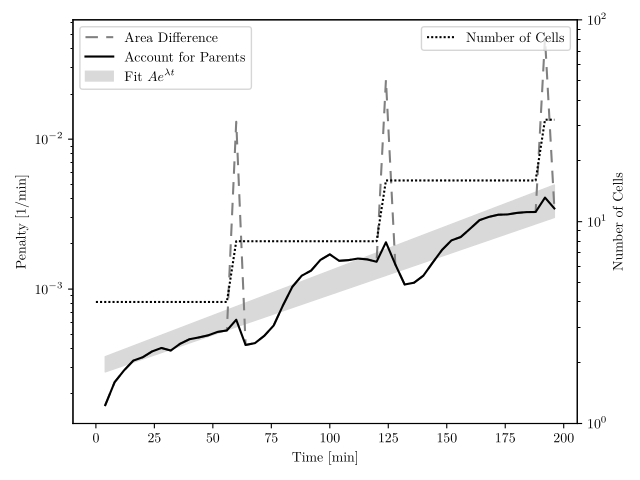
\includegraphics[width=0.5\textwidth]
        {docs/source/_static/fitting-methods/penalty-time-flow.png}%
    \caption{
        Total cost between successive iteration steps $t_n,t_{n+1}$.
        The overall shape is expected to have the slope of an exponential function.
        We can clearly see that division events introduce jumps within this relationship.
        In the case where we account for the parental relationship, these jumps are mitigated.
        The penalty was set to $0$ for pixel-comparisons which belong to cells that are in a
        parental relationship.
    }
    \label{fig:penalty-calculation-cell-division}
\end{figure}

\section{Applications}
% --------------------------------------------------------------------------------------------------
\subsection{A Mechanical Model of Rod-Shaped Bacteria}
\label{subsubsection:mechanical-model-rod-shaped-bacteria}

%###################################################################################################

In order to construct a mechanical model of rod-shaped bacteria, we have to take care of a number of
different aspects.
The mechanical behaviour of rod-shaped bacteria is governed by a plethora of effects.
Although we set out to construct a model which is able to describe as many of these effects as
possible, we will fall short in this paper and restrict ourselves to the aspects presented
in~\ref{table:simulation-aspects}.
We will discuss, how this model can be extended in order to capture more effects and how we can
validate our approach given the existing literaturesection:supplement-more-simulation-aspects
(see section~\ref{section:discussion}, and~\ref{section:supplement-more-simulation-aspects}).

\paragraph{(C) Cellular}
The key component of this model consists of the cellular representation.

It was long believed that bacteria lack cytoskeletal filaments but with the end of the last century,
it was discovered that the MreB protein fills this role since it “[..] forms an actin-like
cytoskeleton in bacteria [..]”~\cite{Erickson2001}.
It can polymerize and form filaments which behave similar to actin microfilaments~\cite{Dersch2020}.
The effect of MreB on the shape of cells during growth was shown in more detail
by~\cite{Ursell2014}.
They found that MreB localizes specifically at regions of negative curvature and thus introduces
heterogeneous cell growth which results in a bending force during the growth of cells.
It also means that the cells are able to sense the curvature of the cell wall through cytoskeleteal
MreB filaments during growth.
\cite{Bratton2018} showed that the trans-membrane protein RodZ can modulate MreB density and
facilitates local MreB assembly.
This feedback mechanism will result in straight rod-shaped bacteria if not interfered from the
external environment.
These results were also confirmed by the studies of~\cite{Wang2010}.
In their experiments, a single bacterium was fixed at the bottom pole while an optically trapped
bead was placed on the upper pole.
They could now exert a force on the free part and thus study the response of the cell under
different conditions.
When treating cells with A22, an antibiotic which disassembles
MreB~\cite{IWAI2002,Gitai2005,Karczmarek2007,Bean2009}, a higher displacement with identical force
could be measured, thus indicating that MreB increases mechanical rigidity of the cell.

While some rod-shaped bacteria grow by inserting new material at the ends, \textit{E.Coli} and
\textit{B.Subtilis} utilize a method where new material is inserted along the cylindrical part of
the rod.
The details of the division event (i.e. Z-Ring formation) are very intricate and are heavily
studied as a subject on their own (TODO citation).
On a higher level view, the rod is split apart at a point close to the center of the cell, thus
creating two new daughter cells.
We know that the best predictor for when the division event occurs, is the length of the rod as
opposed to the age of bacterium~\cite{Robert2014}.
Furthermore, only the growth of the whole colony but also the individual growth of the bacteria is
exponential~\cite{Amir2014,Takeuchi2005}.

\paragraph{(CC) Cell-Cell Interactions \& (DC) Domain-Cell Interactions}
A colony of bacteria is known to form biofilms (Dunne 2002). This strategy is is beneficial for the
survival of the collective as it allows it to harness growth factors and migrate when necessary and
also plays an important role in bacterial infections in the biomedical sector~\cite{Ong1999}.
The formation of biofilms is only possible due to the attractive nature of bacterial interactions
towards each other and surfaces (Berne et al. 2018). To analyze bacterial adhesion to surfaces,
\cite{vanLoosdrecht1989} investigated the interactions of various bacteria with negatively charged
polystyrene.
They found that the interaction is characterized by a low Gibbs energy of $(2 - 3)kT$ per cell
which can be described by a secondary minimum of the DLVO-theory~\cite{Verwey1947,Derjaguin1993}
which is relevant for distances $\geq\SI{1}{\nano\meter}$.
At these distances, the DLVO potential acts as a generic adhesive potential.
Particles which stay in the secondary minimum are held together but even weak interactions are
enough to redisperse them which means that this state is reversible.
When approaching closer distances, more intricate mechanisms come into play in which the
heterogeneity of the materials in question needs to be considered.
\cite{Hori2010} described bacterial adhesion as a “two-phase process including an initial,
instantaneous and reversible physical phase (phase one) and a time-dependent and irreversible
molecular and cellular phase (phase two)”.

All these considerations become even more intricate when not considering interactions of bacteria
with surfaces but bacteria with each other.
Gram-negative bacteria (eg. E.Coli) express outer membrane proteins (adhesins) which allow them to
attach to various hosts (Beachey 1981, Vaca et al. 2019).
In addition, the flagella can play an important role in the direct adhesion between
cells~\cite{Haiko2013}.
Thus it is not correct to blindly apply the results for adhesion to surfaces to the interactions
between bacteria.

\begin{table}
    \centering
    \def\arraystretch{1.3}
    \begin{tabularx}{\textwidth}{c l X}
        &\textbf{Aspect} & \textbf{Description}\\
        \toprule
        &\textbf{(C) Cellular}\\
        \midrule
        (1) & Rod-Shaped Mechanics &
            Rod-shaped bacteria are flexible rods which are able to freely move around (off-lattice
            approach) \cite{Takeuchi2005,Ursell2014,Amir2014_2}.\\
        (2) & Growth &
            Cells grow exponentially by inserting new material along the circular part of the rod
            \cite{Robert2014,Takeuchi2005}.\\
        % (3) & Differentiation &
        %     \textit{B.subtilis} is known to differentiate into matrix-producing and
        %     surfactin-producing cells \cite{vanGestel2015,Lpez2010}.\\
        (3) & Division &
            Rod-Shaped bacteria divide in the middle of the rod, thus forming two new
            agents.
            Bacteria can form multilayers during their growth phase \cite{Duvernoy2018}.\\
        (4) & Variable Parameters &
            Parameters for individual cells are not fixed values but rather taken from a
            distribution \cite{Koutsoumanis2013}.\\
        &\textbf{(CC) Cell-Cell Interactions}\\
        \midrule
        (5) & Adhesion &
            Bacteria adhere to each other at longer distances and attach when in close contact
            \cite{Verwey1947,Trejo2013}.\\
            % The interaction between rods can be polarized \cite{Duvernoy2018}.\\
        % (7) & Friction &
        %     Friction between cells \cite{Grant2014} can be asymmetrical \cite{Doumic2020}.\\
        &\textbf{(DC) Domain-Cell Interactions}\\
        \midrule
        (6) & External Forces &
            Bacteria which rub against surfaces tend to stick to them after some
            time~\cite{vanLoosdrecht1989}.
            The extracellular gel which surrounds the bacteria exerts a force onto the cells
            \cite{Grant2014}.\\
        % (9) & Extracellular Reactions &
        %     Bacteria can take up nutrients or possible secrete/take up signalling molecules
        %     \cite{Li2025}.\\
        \bottomrule
    \end{tabularx}
    \label{table:simulation-aspects}
    \caption{TODO Insert caption}
\end{table}

To model the spatial mechanics of elongated bacteria \cite{Billaudeau2017}, we represent them as a
collection of auxiliary vertices $\{\vec{x}_i\}$ which are connected by springs in
ascending order.
Furthermore, we assume that the cells are flexible described by their rigidity.
A force $\vec{F}$ interacting between cellular agents determines the radius (thickness) of the
rods and an attractive component can model adhesion between cells.

% --------------------------------------------------------------------------------------------------
\subsection{Mechanics}
\label{subsection:mechanical-model-mechanics}

We use principles from discrete differential geometry~\cite{bobenko2008discrete} to describe the
stiffness and flexibility of the bacterial rod.
As explained previously, MReB will counteract the bending of the rod, resulting in a stiffening
force.
In order to construct a model which can be parametrized and by method of Occam's Razor, we chose to
model the bacterium as a bending beam, thus utilizing the simplest solution which can still produce
the desired effects.
Such a beam can be represented by a collection of vertices $\vec{x}_i$ which are connected by a
springs of lengths $l_i$.
We use the notation $\vec{c}_i:=\vec{x}_i-\vec{x}_{i-1}$ with which the resulting force acting
between two vertices if given by

\begin{align}
    \vec{F}_{i,\text{springs}} =
        &-\gamma\left(1 - \frac{l}{\left|\vec{c}_i\right|}\right)
        \vec{c}_i\\
        &+ \gamma\left(1 - \frac{l}{\left|\vec{c}_{i+1}\right|}\right)
        \vec{c}_{i+1}.
\end{align}

In addition to springs between individual vertices $\vec{x}_i$, we assume that each angle at a
vertex between edges is subject to a force indiced by curvature.
% We assume that we can model the mechanical properties of the bacterium as an elastic rod.
Given the angle $\alpha_i = \sphericalangle(\vec{c}_{i-1},\vec{c}_i)$ between adjacent edges,
the bending force is proportional to the curvature $\kappa_i$ at each vertex
$\kappa_i = 2\tan(\alpha_i/2)$.
The resulting force acts along the angle bisector which can be calculated from the edge vectors.
Figure~\ref{fig:mechanics-bacterium} shows an elongated rod represented by $6$ vertices.
The forces acting on vertices $\vec{x}_i,\vec{x}_{i-1},\vec{x}_{i+1}$ are given by

\begin{align}
    \vec{F}_{i,\text{curvature}} &= \eta\kappa_i
        \frac{\vec{c}_i - \vec{c}_{i+1}}{|\vec{c}_i-\vec{c}_{i+1}|}\\
    \vec{F}_{i-1,\text{curvature}} &= -\frac{1}{2}\vec{F}_{i,\text{curvature}}\\
    \vec{F}_{i+1,\text{curvature}} &= -\frac{1}{2}\vec{F}_{i,\text{curvature}}
\end{align}

where $\eta_i$ is the rigidity at vertex $\vec{x}_i$ (see Figure~\ref{fig:mechanics-bacterium}).
We can see that the curvature force does not move the overall center of the rod in space.
The total force is the sum of external and interal forces.

\begin{equation}
    \vec{F}_{i,\text{total}} = \vec{F}_{i,\text{springs}}+ \vec{F}_{i,\text{curvature}}
        + \vec{F}_{i,\text{external}}
\end{equation}

and are integrated via

\begin{align}
    \partial_t^2 \vec{x}_i &= \partial_t\vec{x}_i + \sqrt{2D}\vec{\xi}_i\\
    \partial_t\vec{x}_i &= \vec{F}_{i,\text{total}} - \lambda \partial_t\vec{x}_i
\end{align}

where $D$ is the diffusion constant and $\vec{\xi}$ is the wiener process.
Together they determine the stochastic motion of the individual vertices which can arise from
recurring collisions with small particles of the surrounding medium or other minor fluctuations.

%TODO use these citations
\cite{Chatterjee1988},\cite{Ursell2014}

% --------------------------------------------------------------------------------------------------
\subsection{Interactions}
\label{subsection:mechanical-model-interactions}

When calculating forces acting between the cells, we can use a simplified model to circumvent the
numerically expensive integration over the complete length of the rod.
Given a vertex $\vec{x}_i$ on one cell, we calculate the closest point $\vec{p}$ on the polygonal
line given by the vertices $\{\vec{w}_j\}$ of the interacting cell.
Furthermore we determine the value $q\in[0,1]$ such that $\vec{p} = (1-q)\vec{w}_j + q\vec{w}_{j+1}$
for some specific $j$.
The force is then calculated between the points $\vec{x}_i$ and $\vec{p}_i$ and acts on
the vertex $\vec{w}_i,\vec{w}_{i+1}$ with relative strength $(1-q)$ and $q$.

\begin{equation}
    \vec{F}_{i,\text{External}} = \vec{F}(\vec{x}_i,\vec{p})
    \label{eq:cell-force-external}
\end{equation}

The specific choice of interaction potential plays of course a crucial role for the dynamics of the
agents.
But we cannot expect to simply know the shape and parameters of this potential.
Thus, we would like to experiment with various interaction potentials in order to quantify their
ability to produce accurate results.
We utilize two distinct potentials that are both able to capture the essence of our interactions by
providing a short-range repulsive part and a long-ranged attractive component.

\paragraph{Morse Potential}
The morse potential~\cite{Morse1929} is a common example of numerically inexpensive interaction
potential.
It was originally designed to describe the interaction of diatomic molecules but has since found use
in other areas~\cite{Breitwieser2021}.
It contains a repulsive and attractive part and is bound from above which makes it particularly
suitable for numerical simulations since unbound potentials can lead to large numerical deviations
thus compromising the prediction of the model.
The potential is of the form
\begin{equation}
    V(r) = V_0\left(1-e^{-\lambda(r-(R_1+R_2))}\right)^2
\end{equation}
and has 3 parameters.
The overall potential strength $V_0$, the radii of the particles $R_1,R_2$ and the potential
stiffness $\lambda$ which controls the rate of change as one travels along the radial axis.
We employ a spatial cutoff which sets the interaction strength to $0$ when exceeding a distance
$r\geq\xi$.

\paragraph{Mie Potential}
The Mie~\cite{Mie1903} potential is the generalization of the well-known
Lennard-Jones~\cite{Jones1924} potential.
It was also designed to describe the interactions of molecules but due to the flexible nature of its
parameters, can be easily adapted to other situations.
It is able to describe a wider range of shapes compared to the Morse potential but is also stiffer
and not bound from above.
In our simulation, we enforce an upper bound to guarantee numerical regularity.
It has 4 parameters and is given by
\begin{align}
    U(r) &= C\epsilon\left[ \left(\frac{\sigma}{r}\right)^n -
        \left(\frac{\sigma}{r}\right)^m\right]\\
    C &= \frac{n}{n-m}\left(\frac{n}{m}\right)^{\frac{n}{n-m}}\\
    V(r) &= \min(U(r), \beta)\theta(r-\zeta)
\end{align}
where $C$ is a constant that depends on the two exponents $n,m$ that describe the overall shape of
the potential.
The strength is given by $\epsilon$ and the radius is encoded in $\sigma =
(m/n)^{1/(n-m)}(R_1+R_2)$ where $R_1,R_2$ are the radii of the two interacting particles.

% --------------------------------------------------------------------------------------------------
\subsection{Cycle}
\label{subsection:mechanical-model-cycle}

To simulate proliferation, we introduce a growth term for the spring lengths $l_i$.
In most of our simulations, we choose to use identical lengths for all segments (i.e. $l_i=l$).
However, in order to generalize our approach we assume that individual lengths of segments could
vary.
We reduce the growth rate with increasing number of neighbors $N$.
This behaviour can be toggled on or off thus removing the additional term in brackets of
equation~\ref{eq:growth-rod-lengths}.

\begin{equation}
    \partial_t l_i = \mu\left(1-\frac{\text{min}(n,N)}{N}\right)l_i
    \label{eq:growth-rod-lengths}
\end{equation}

Note that the growth rate is proportional to the rod length $l$ which leads to exponential growth.
This process will increase the length of the cell indefenitely unless we impose a condition for the
division event.
We define a fixed length threshold for the total length of the cell at which it divides.
To construct a new cell, we cannot simply copy the existing one twice, but we also need to adjust
internal parameters in the process.
The following actions need to be taken for the old and new agent.
We first calculate the new spring lengths of the two resulting rods.
\begin{equation}
    \tilde{l} = l_i\left(\frac{1}{2} - \frac{r}{\sum\limits_i l_i}\right)
    \label{eq:growth-rod-new-lengths}
\end{equation}
Afterwards, we start at one endpoint $\vec{v}_0$ and travel along the polygon defined by the
bacterial rod.
We stop when we have reached a length that matches the length of the new spring length $\tilde{l}$.
From here, we continue and iterate this procedure until we have found all new vertices $\vec{w}_i$.
Equation~\ref{eq:growth-rod-new-lengths} ensures that that the tips of the two new rods are touching
right after the division event.

% --------------------------------------------------------------------------------------------------
\subsection{External Forces}
\label{subsection:mechanical-model-external-forces}
TODO
\begin{itemize}
    \item Friction force against surface. perpendicular to motion; proportional to velocity.
    \item gel pressure coming from experiment (simply downwards force $F_z$)
\end{itemize}

% --------------------------------------------------------------------------------------------------
\subsection{Numerical Implementation}

We implemented the described model in \texttt{cellular\_raza}~\cite{Pleyer2025}.
Doing so has many benefits.
Not only, was a more simpler model already available which could be adapted to our needs.
But furthermore, due to the nature of \texttt{cellular\_raza} in that it does not assume any
particular cellular representation, we are free to change the underlying model at any time, even
making fundamental changes.
It is an \ac{abm} which is able to natively track cells through the course of a numerical simulation
and also keeps track of parent/daughter relationships.
This allows us to to experiment with different model implementations and still retain performance.
By leveraging the strong safety guarantees provided by the Rust programming language, we eliminate a
whole class of problems from the start.
% TODO CITATION
In addition, we are using the \texttt{pyo3} and \texttt{maturin} crates which allow us to easily
generate python bindings and thus interoperate between the two ecosystems.
While this particular model is more complex due to the nature of non-trivial (asymmetric)
interactions, we were still able to properly utilize the speedup from executing simulations in
parallalel using the built-in parallelization methods of \texttt{cellular\_raza} (see
Supplementary Material, Figure~\ref{fig:performance}).

% --------------------------------------------------------------------------------------------------
\subsection{Estimating Mechanical Parameters of Growing \textit{E.Coli.} on Agar}
We will now focus on using the presented methods for parameter estimation via microscopic images.
Our initial state is given by TODO~\cite{}.% TODO
We use our extraction algorithm to obtain the initial positions of our cells.
From there, we supply the model with parameters such that we can make a prediction for the final
positions of the bacteria.
We chose a time-interval which does not contain any division events.
By doing so, we can utilize the simpler and more performant position comparison scheme for our cost
function.
Another important detail is the individuality of the agents.
In our case, this means that each agent might have different parameters associated to it.
For this dataset, we assumed that all interaction parameters which specify the interaction
potential are identical across all agents but growth rates and the physical radii of the cells are
individual and we also optimize them.
We chose to optimize for 3 interaction parameters of the Mie potential $n,m,V_0$ and two parameters
which were individual for each cell, namely the radii $r_i$ and growth rates $\mu_i$.
We also included the damping constant $\lambda$ and removed any stochastic motion contributions
($D=0$).
This leads to a total of $4+2\times 6=16$ parameters.
To estimate these parameters we used a latin-hypercube sweep across the parameter space and
performed a local minimization with the Nelder-Mead method (TODO citations).% CITATIONS

Figure~\ref{fig:parameter-estimates-single-step} shows the cost function of multiple simulations.
The curves show the value at the found optimium and how it changes when varying the value of the
parameter in question.
We have exemplified the values for radii $r_i$ and growth rates $\mu_i$ with values of the first
cell.
The remaining plots can be found in the supplementary material in
section~\ref{sec:supplement-parameter-profiles}.

This depiction is similar to the method of profile likelihood~\cite{Raue2009}.
We can see that almost all parameters can be estimated by our optimization approach.
However, the damping constant exhibits the well-known phenomenon of
unidentifiability~\cite{Raue2009}.
This is of course problematic since the real value of $\lambda$ can not be idenified in this case.
But it also shows that the approach which we used is similar in its ability to detect these defects
in the first place.
As we continue to develop these methods, we expect to be able to reuse many of the existing
theoretical approaches which have already been developed for less complex systems such as \acp{ode}.
Fortunately, \texttt{cellular\_raza} was chosen to construct our model such that we are flexible in
changing the underlying representation if should find that such unidentifiabilities are structural
(model-based) rather than practical (due to lack of data).
This allows us to iterate and find the model formulation which suits the data best but still retain
the mechanistic methodology of our approach.

\begin{figure}[H]
    \centering
    \begin{tikzonimage}[width=0.33\textwidth]
        {figures/crm_fit/profiles/damping.pdf}%
        \node at (0.025, 0.975)[anchor=north west, rectangle, draw, black, minimum width=15pt, minimum height=15pt]{\textbf{A}};
    \end{tikzonimage}%
    \begin{tikzonimage}[width=0.33\textwidth]
        {figures/crm_fit/profiles/exponent-m.pdf}%
        \node at (0.025, 0.975)[anchor=north west, rectangle, draw, black, minimum width=15pt, minimum height=15pt]{\textbf{B}};
    \end{tikzonimage}%
    \begin{tikzonimage}[width=0.33\textwidth]
        {figures/crm_fit/profiles/exponent-n.pdf}%
        \node at (0.025, 0.975)[anchor=north west, rectangle, draw, black, minimum width=15pt, minimum height=15pt]{\textbf{C}};
    \end{tikzonimage}\\
    \begin{tikzonimage}[width=0.33\textwidth]
        {figures/crm_fit/profiles/strength.pdf}%
        \node at (0.025, 0.975)[anchor=north west, rectangle, draw, black, minimum width=15pt, minimum height=15pt]{\textbf{D}};
    \end{tikzonimage}%
    \begin{tikzonimage}[width=0.33\textwidth]
        {figures/crm_fit/profiles/growth-rate-0.pdf}%
        \node at (0.025, 0.975)[anchor=north west, rectangle, draw, black, minimum width=15pt, minimum height=15pt]{\textbf{E}};
    \end{tikzonimage}%
    \begin{tikzonimage}[width=0.33\textwidth]
        {figures/crm_fit/profiles/radius-0.pdf}%
        \node at (0.025, 0.975)[anchor=north west, rectangle, draw, black, minimum width=15pt, minimum height=15pt]{\textbf{F}};
    \end{tikzonimage}
    \caption{
        The curves show the value of the cost function at the optimium as determined by our
        otimization scheme (blue dot).
        We have chosen a single parameter and calculated the resulting cost function across a range
        of values and plotted it.
        In the cases of (B-F), we can see that a minimum was achieved and thus the parameters could
        be identified.
        However, for the case of the damping constant $\lambda$ in (A), a non-identifiability
        arises.
    }
    \label{fig:parameter-estimates-single-step}
\end{figure}

% --------------------------------------------------------------------------------------------------
\subsection{Data Generation}

%###################################################################################################
\section{Discussion}
\label{section:discussion}

\begin{itemize}
    \item Model does not capture every aspect of rod-shaped bacteria. Needs to extended (see our
        review).
    \begin{enumerate}
        \item polar interactions
        \item differentiation for van Gogh bundles; surfactin-producing, matrix-producing cells.
        \item Proper friction; this might have a huge implication on the estimation of
            parameters~\cite{Grant2014}.
            This paper has already implemented this~\cite{Doumic2020}.
            We can build on top of that.
        \item Extracellular Reactions~\cite{Li2025}
        \item see supplement for full list \ref{table:simulation-aspects-supplement}
    \end{enumerate}
    \item Data Extraction: Skeletonization Algorithm ultimately not good enough for some scenarios
        (i.e. overlapping of cells, endpoints can sometimes be "too short")
    \begin{itemize}
        \item Possibly use AI for new algorithm
    \end{itemize}
    \item Image generation; Produce high-quality near-realistic microscopic images with cell-masks
        from scratch with mechanistic model; train cell-segmentation and more importantly
        cell-tracking algorithms with that.
\end{itemize}

\section{Conclusion}
\label{section:conclusion}

\begin{itemize}
    \item Highlight methodological advancements
    \item Constructed Model which already combines many effects; extend this even further
    \item Proof of concept: Able to fit individual parameters of the agents; can be extend this?
    \item Provide software package which combines all functionality and is readily available
\end{itemize}

%###################################################################################################
% EXCLUDE THIS FOR NOW
% \section{Plastic Deformations}
% 
% \begin{figure}[H]
%     \centering
%     \includegraphics[width=0.49\textwidth]
%         {docs/source/_static/scripts/crm_amir/0000000023.png}\\
%     \includegraphics[width=0.49\textwidth]
%         {docs/source/_static/scripts/crm_amir/angles.pdf}
%     \includegraphics[width=0.49\textwidth]
%         {docs/source/_static/scripts/crm_amir/endpoints.pdf}
%     \caption{TODO}
%     \label{fig:amir}
% \end{figure}

\bibliographystyle{IEEEtran}
\bibliography{references}

%###################################################################################################
\section*{Supplementary Material}

\renewcommand{\thesection}{S\arabic{section}}
\setcounter{section}{0}

%###################################################################################################
\section{Parameter Estimation}
\label{sec:supplement-parameter-profiles}
%TODO {explain profiles}
\begin{figure}[H]
    \centering
    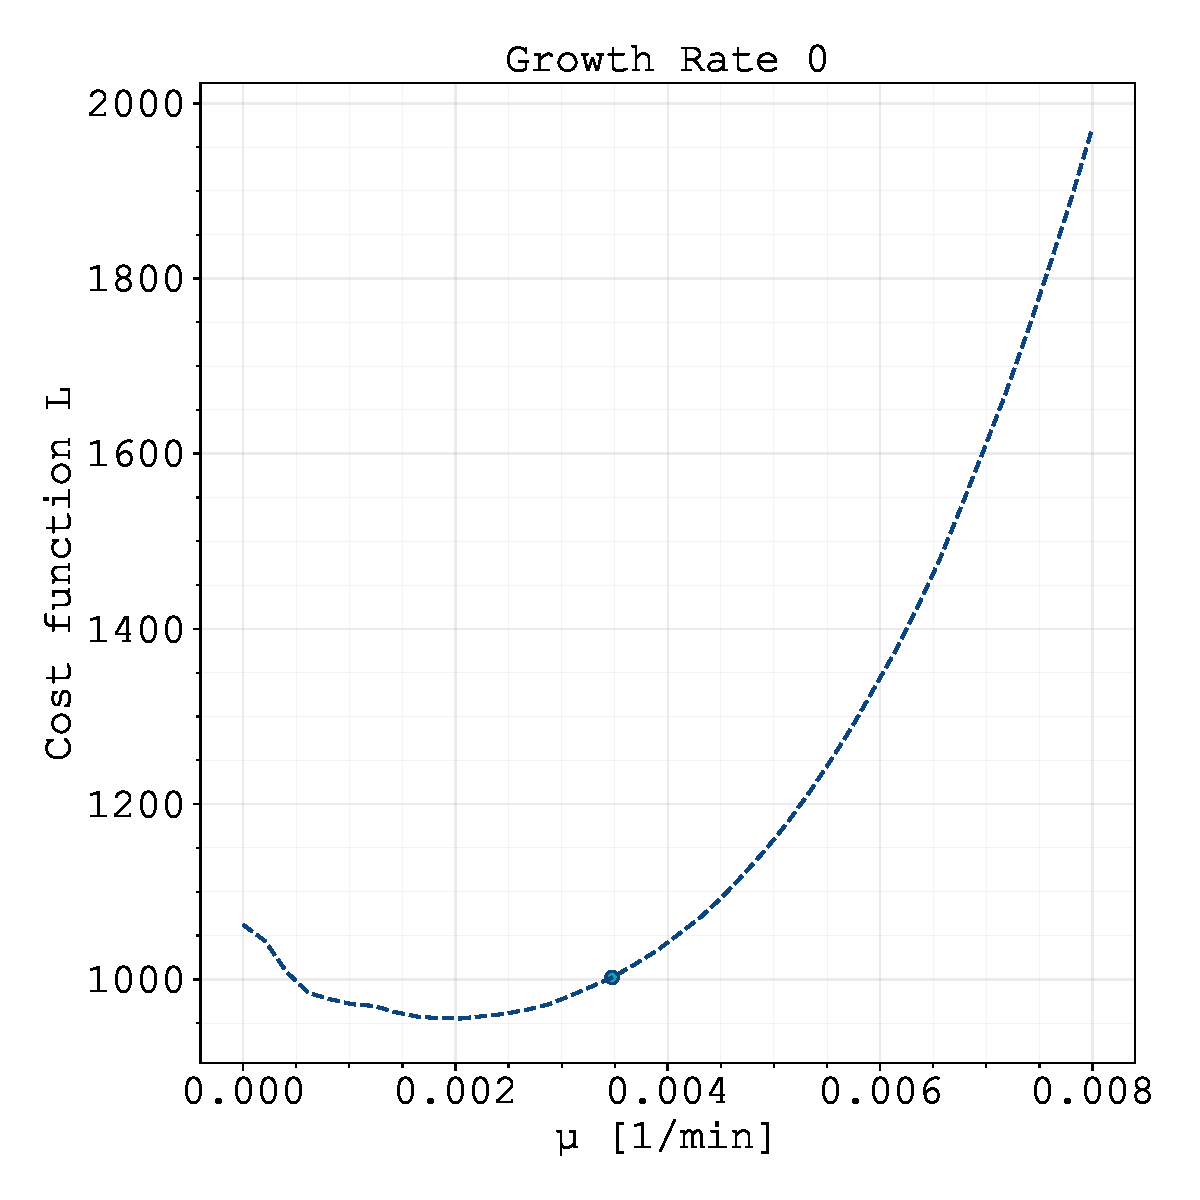
\includegraphics[width=0.33\textwidth]
        {figures/crm_fit/profiles/growth-rate-0.pdf}%
    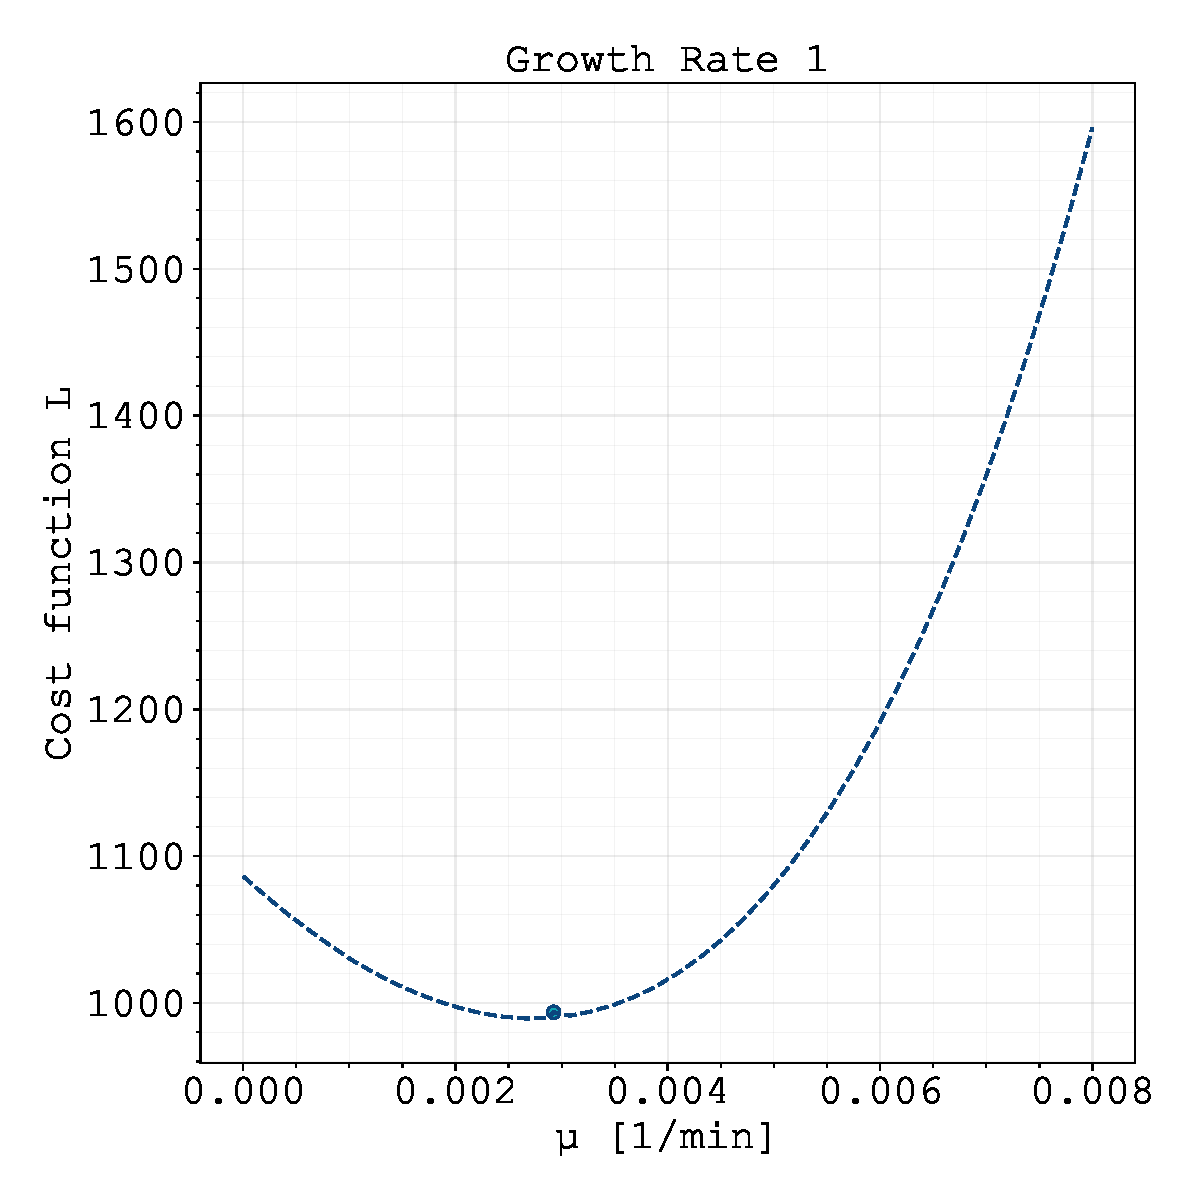
\includegraphics[width=0.33\textwidth]
        {figures/crm_fit/profiles/growth-rate-1.pdf}%
    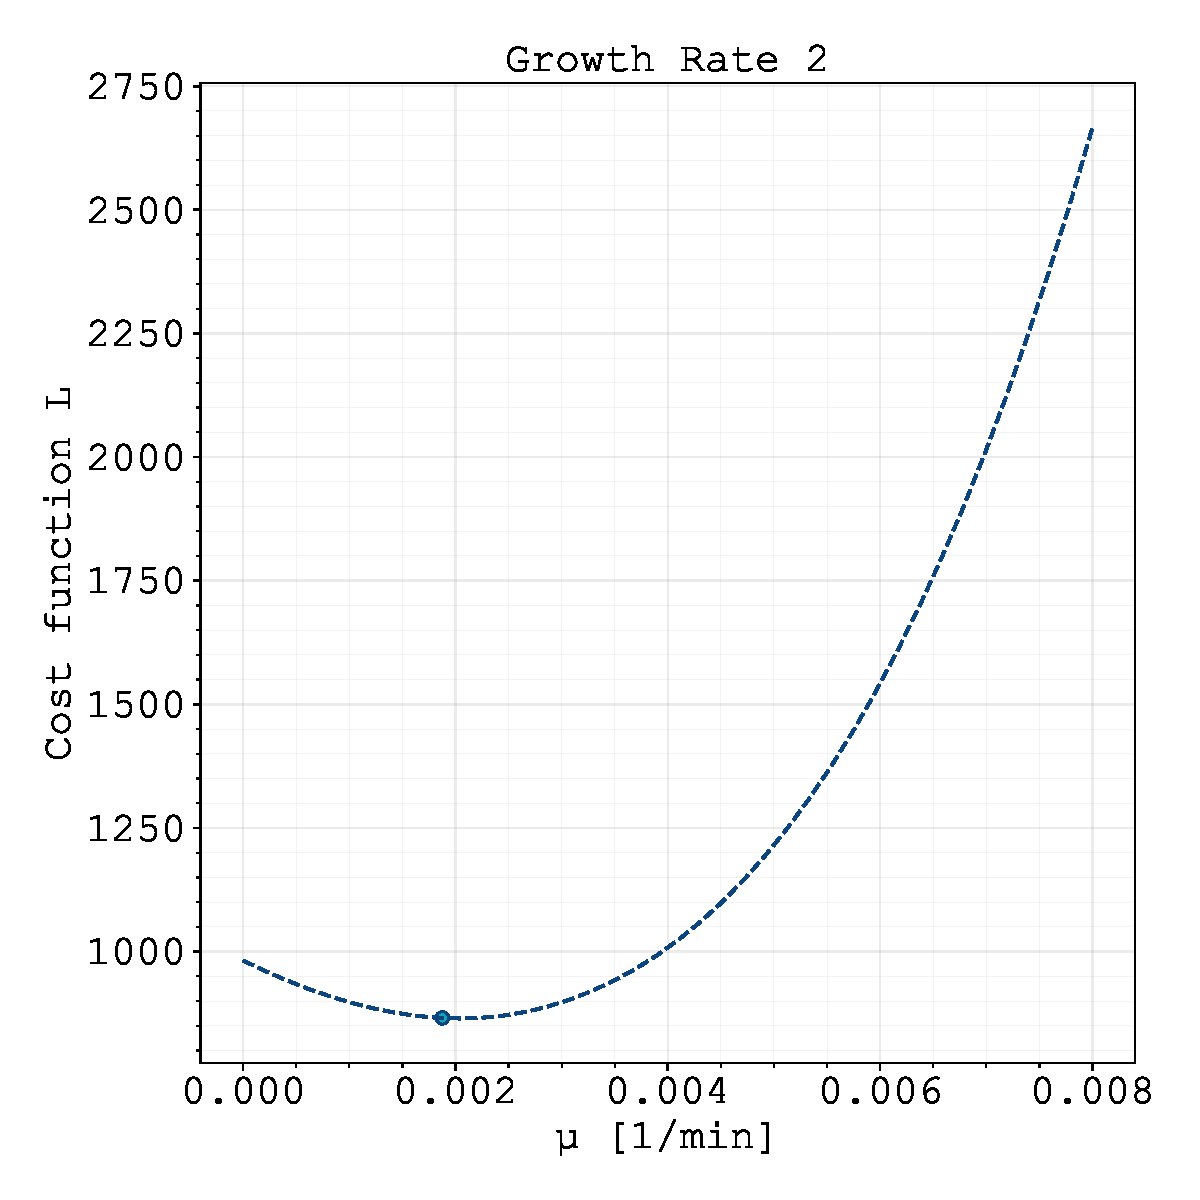
\includegraphics[width=0.33\textwidth]
        {figures/crm_fit/profiles/growth-rate-2.pdf}\\%
    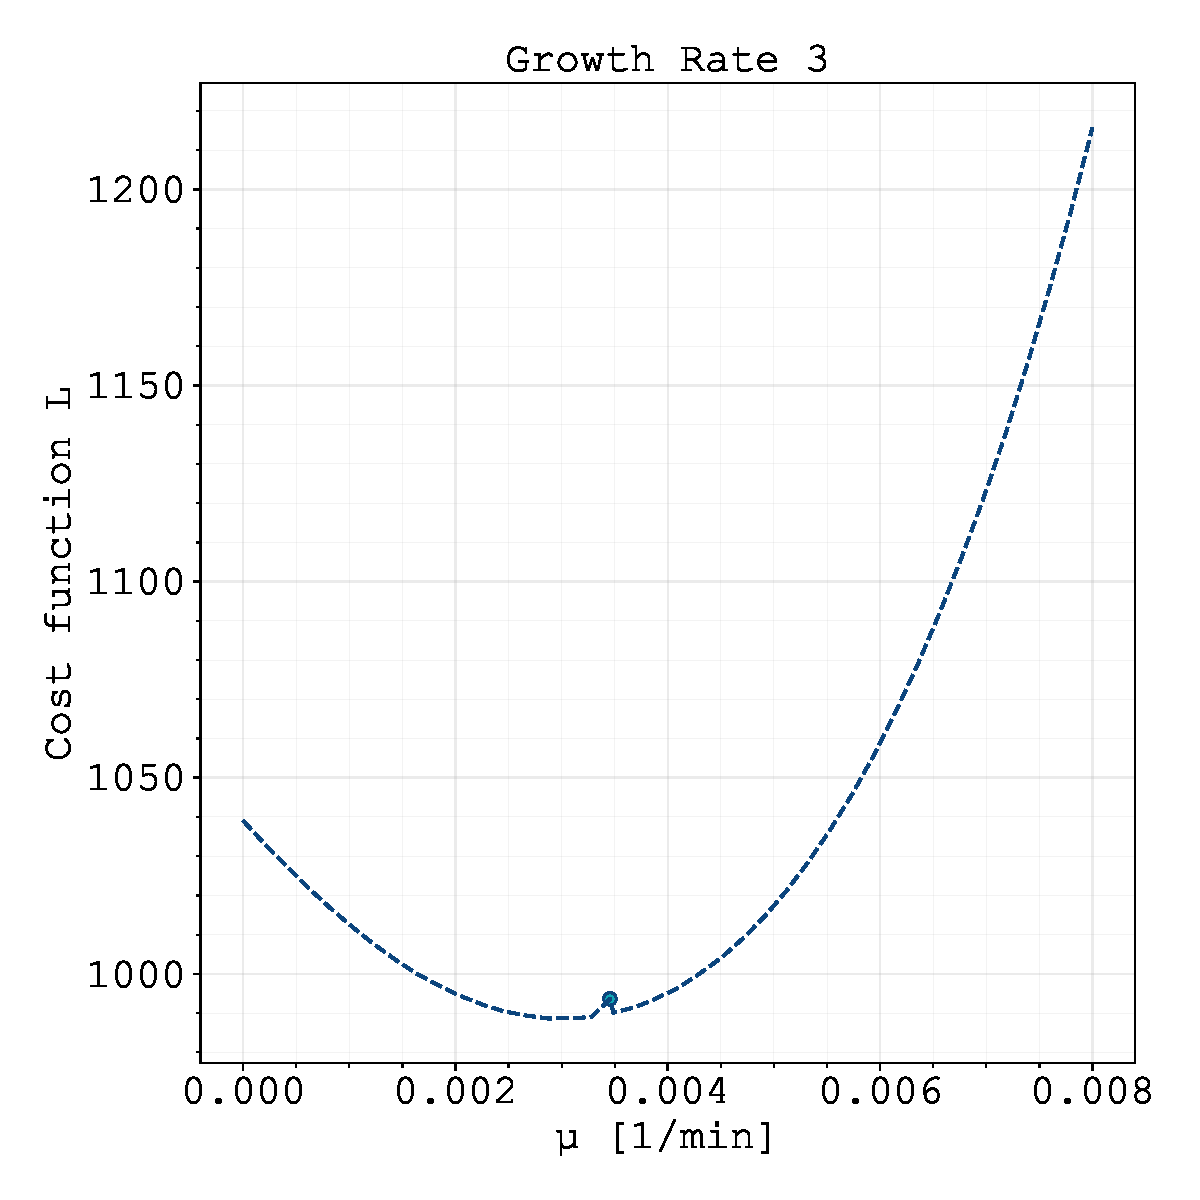
\includegraphics[width=0.33\textwidth]
        {figures/crm_fit/profiles/growth-rate-3.pdf}%
    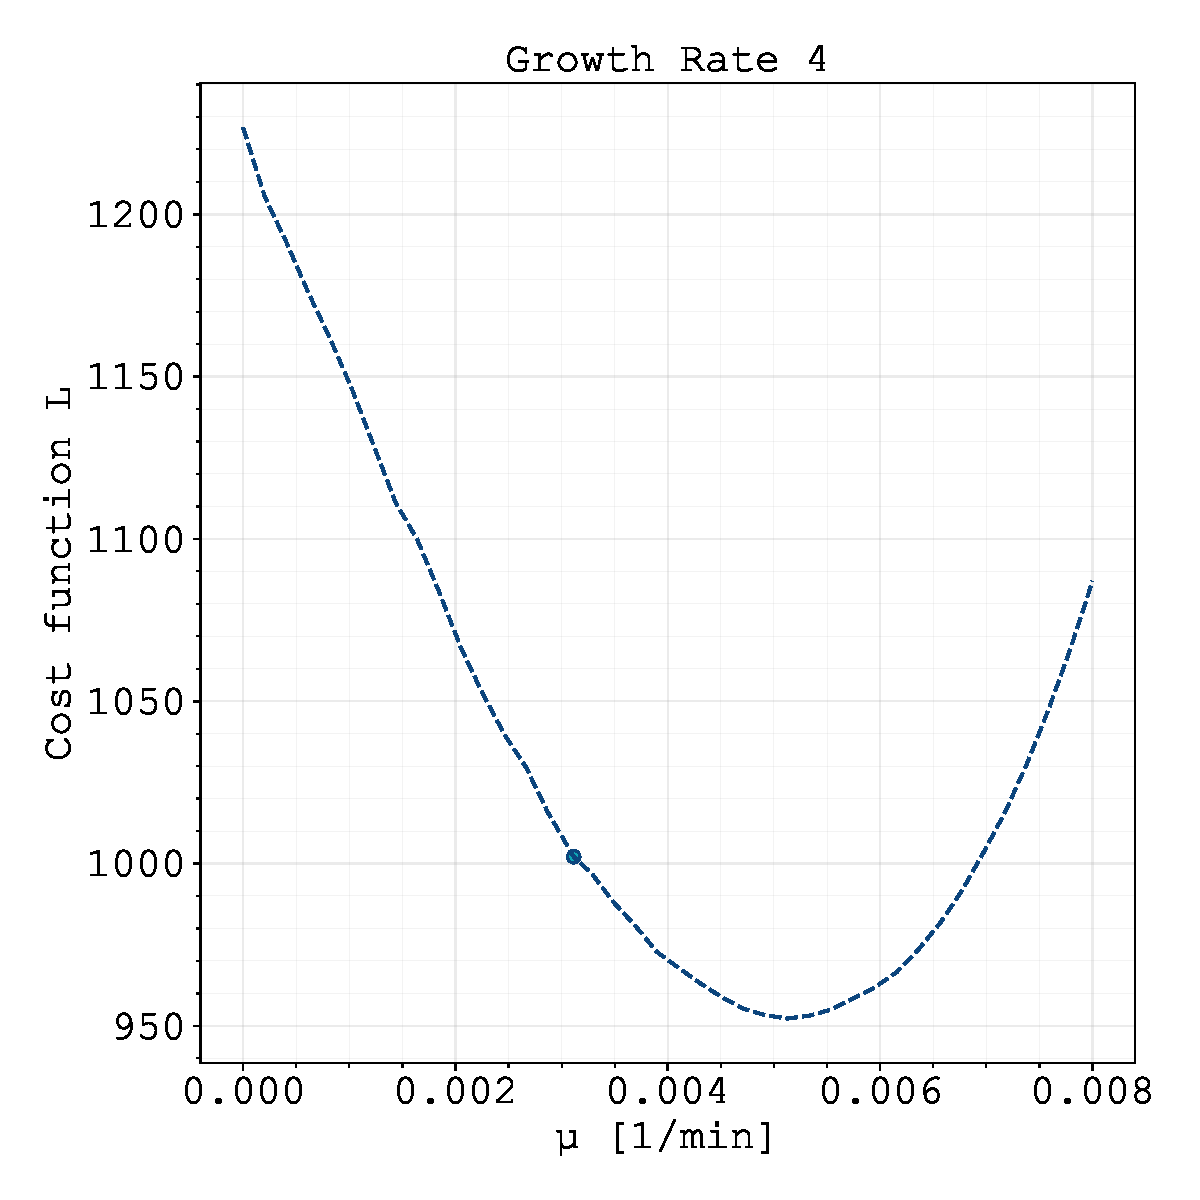
\includegraphics[width=0.33\textwidth]
        {figures/crm_fit/profiles/growth-rate-4.pdf}%
    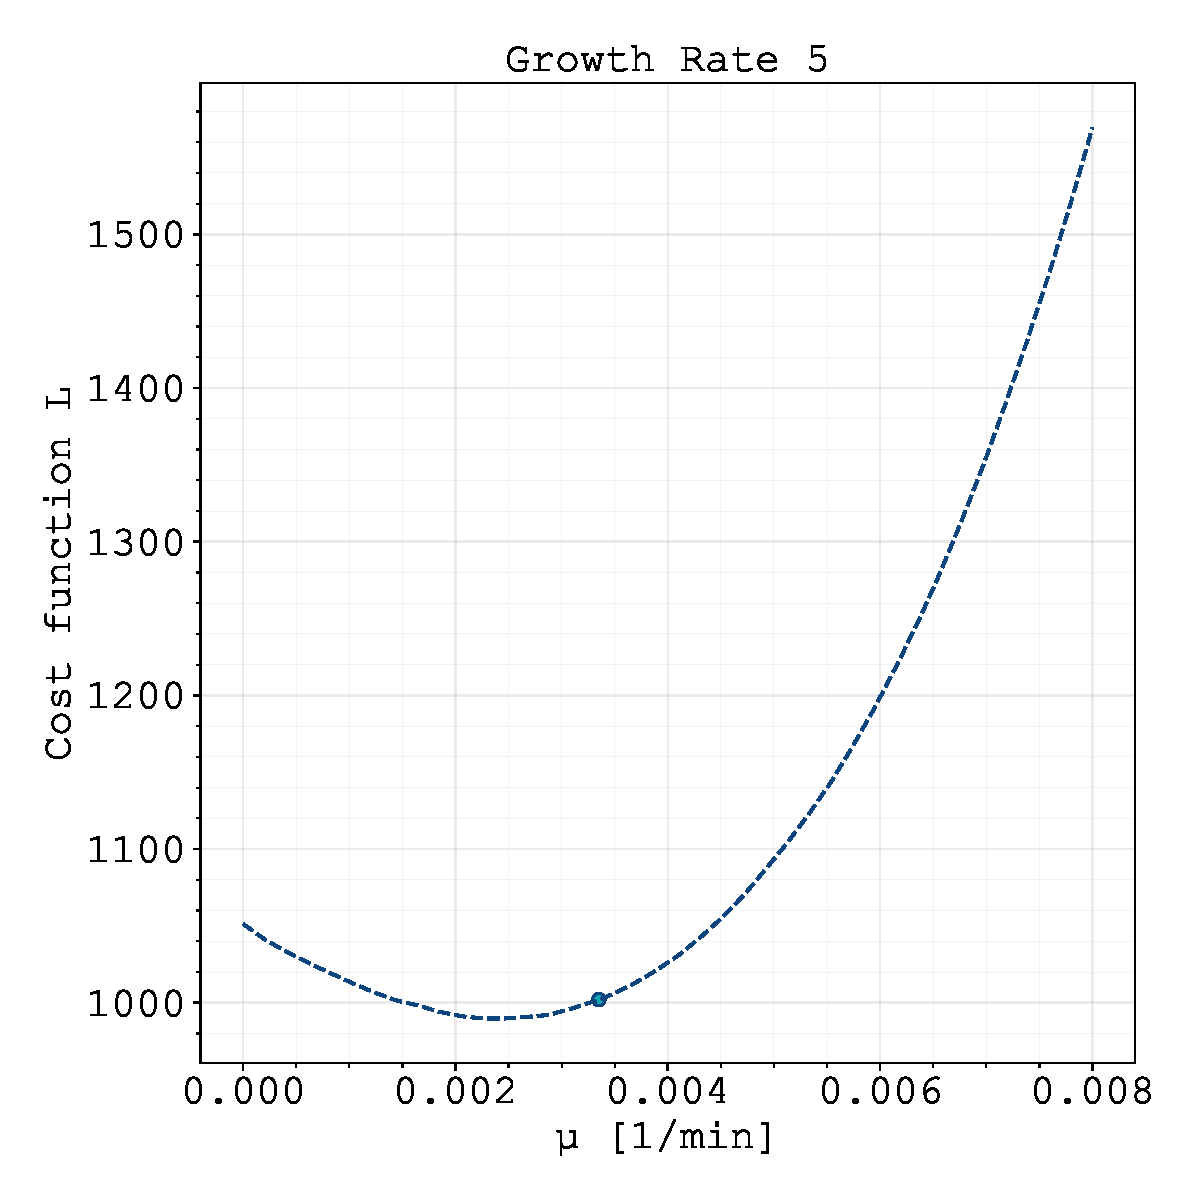
\includegraphics[width=0.33\textwidth]
        {figures/crm_fit/profiles/growth-rate-5.pdf}
    \caption{Parameter estimation of growth rates for individual cells}%TODO extend caption}
    \label{fig:parameter-estimates-supplement-growth-rates}
\end{figure}
\begin{figure}[H]
    \centering
    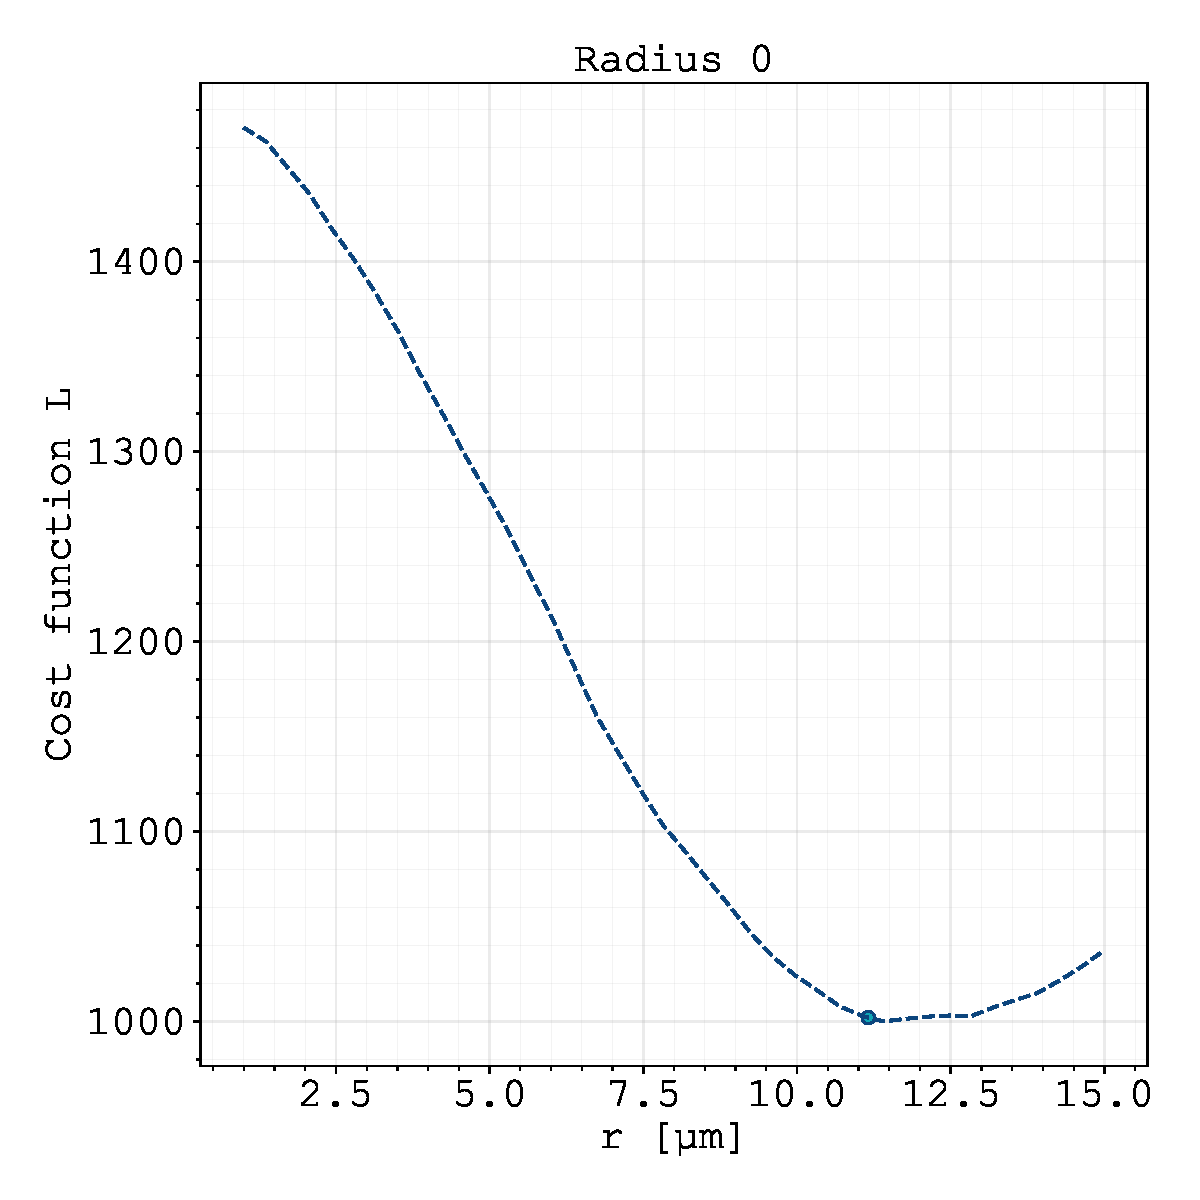
\includegraphics[width=0.33\textwidth]
        {figures/crm_fit/profiles/radius-0.pdf}%
    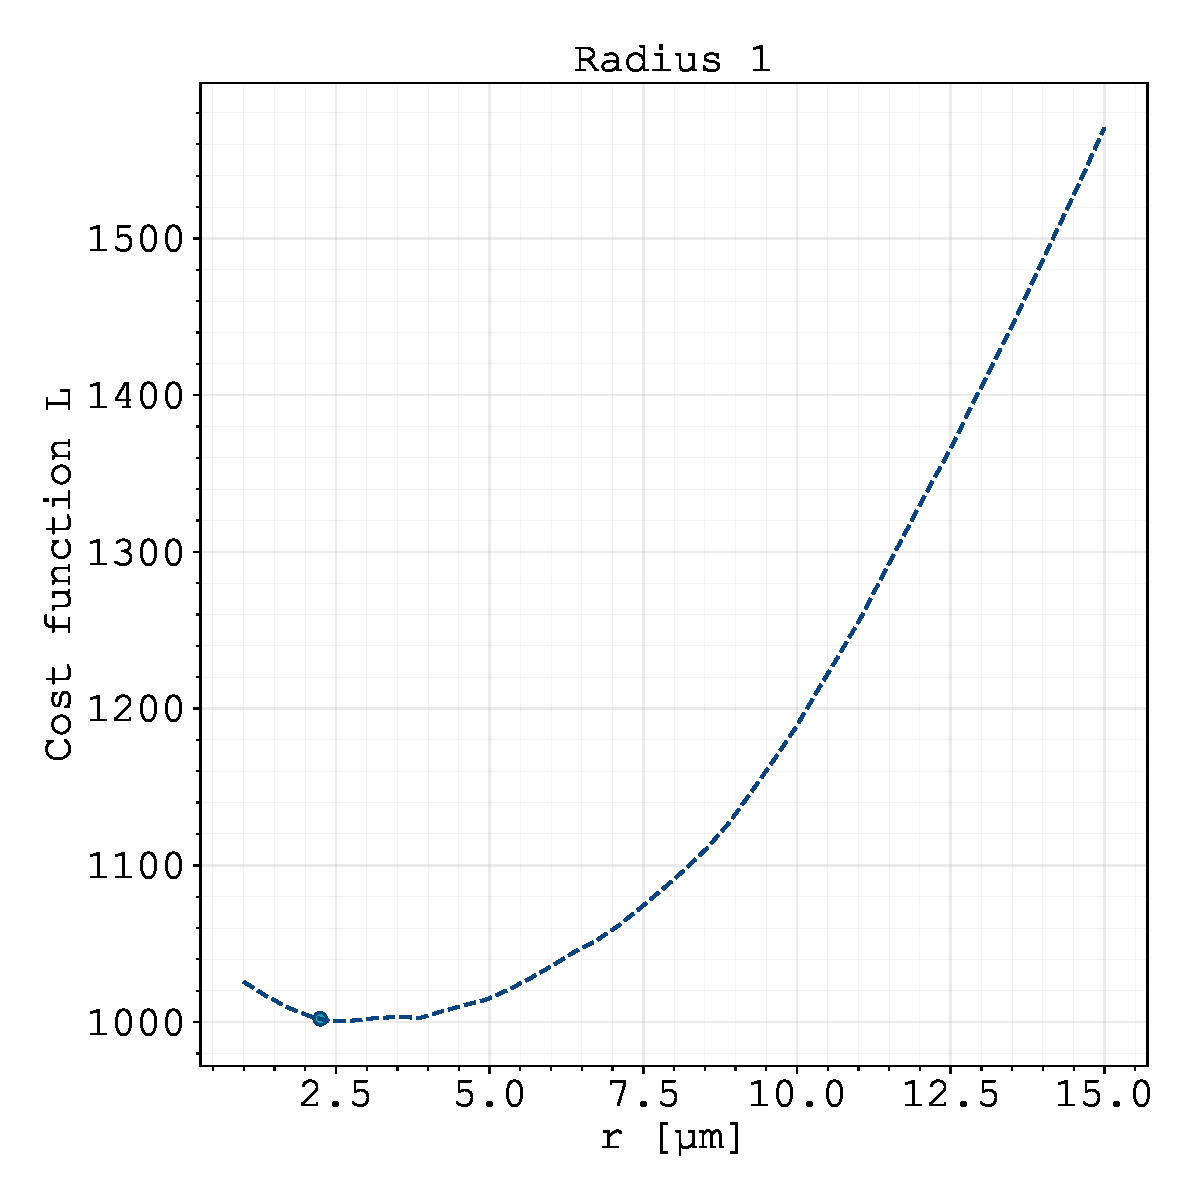
\includegraphics[width=0.33\textwidth]
        {figures/crm_fit/profiles/radius-1.pdf}%
    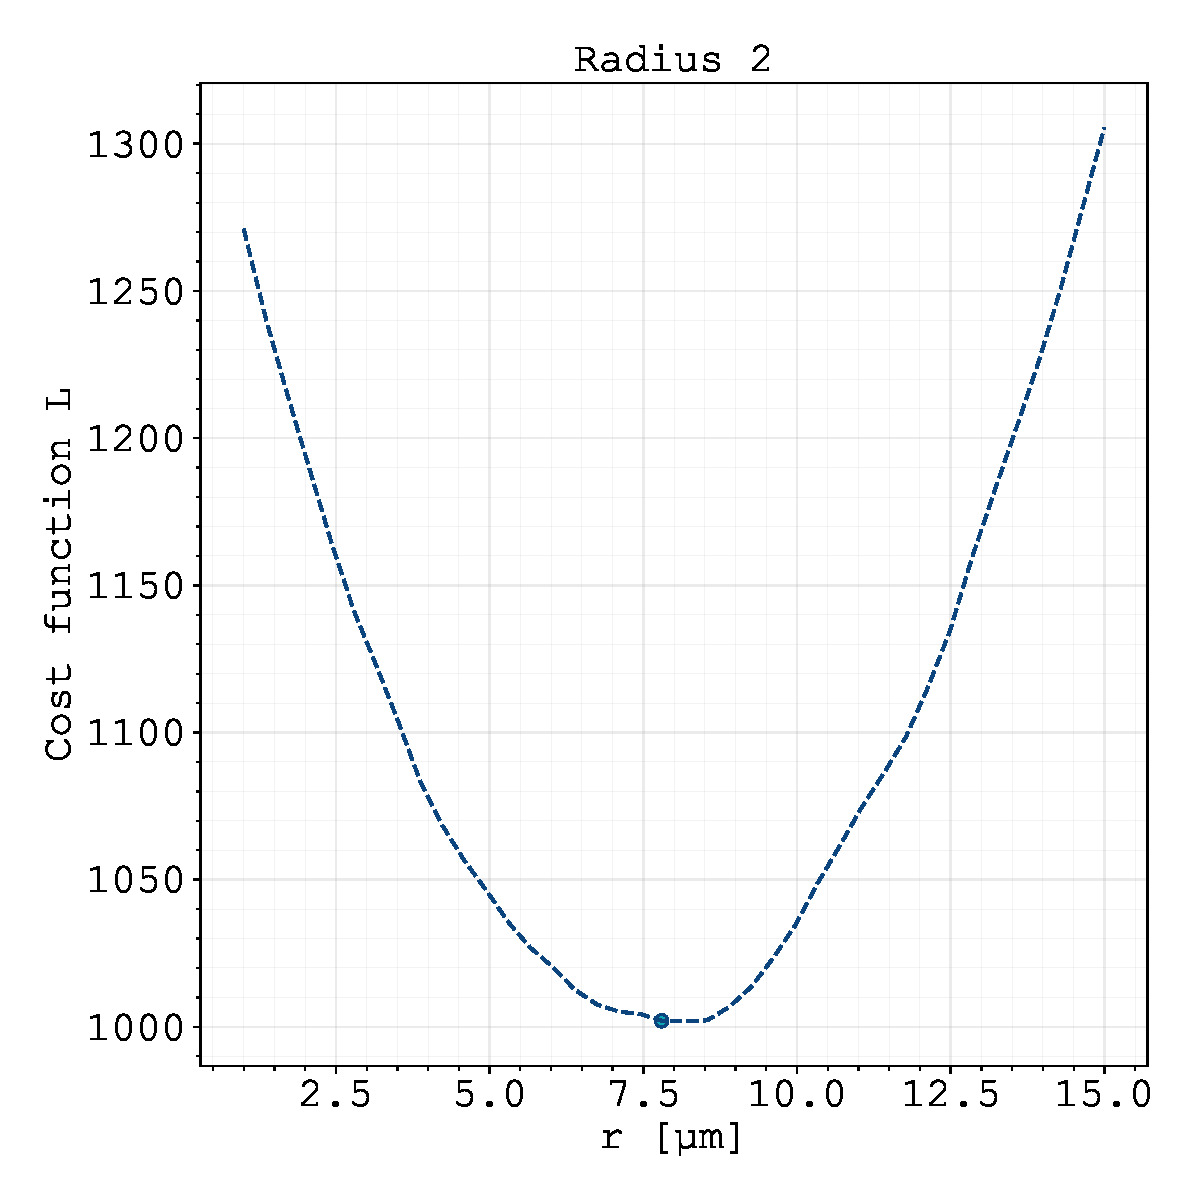
\includegraphics[width=0.33\textwidth]
        {figures/crm_fit/profiles/radius-2.pdf}\\%
    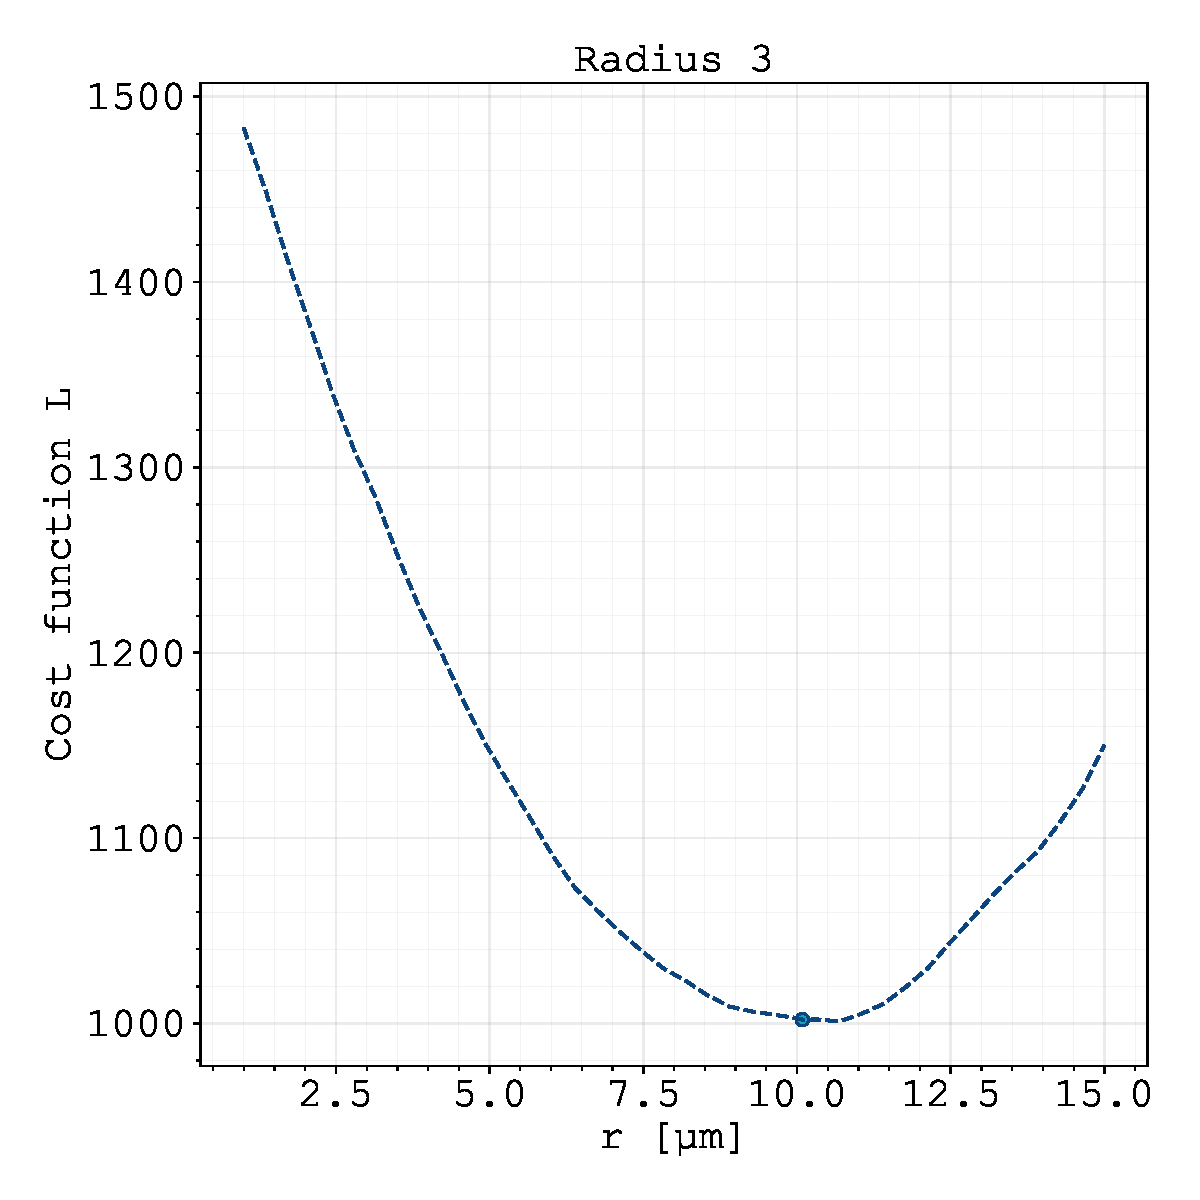
\includegraphics[width=0.33\textwidth]
        {figures/crm_fit/profiles/radius-3.pdf}%
    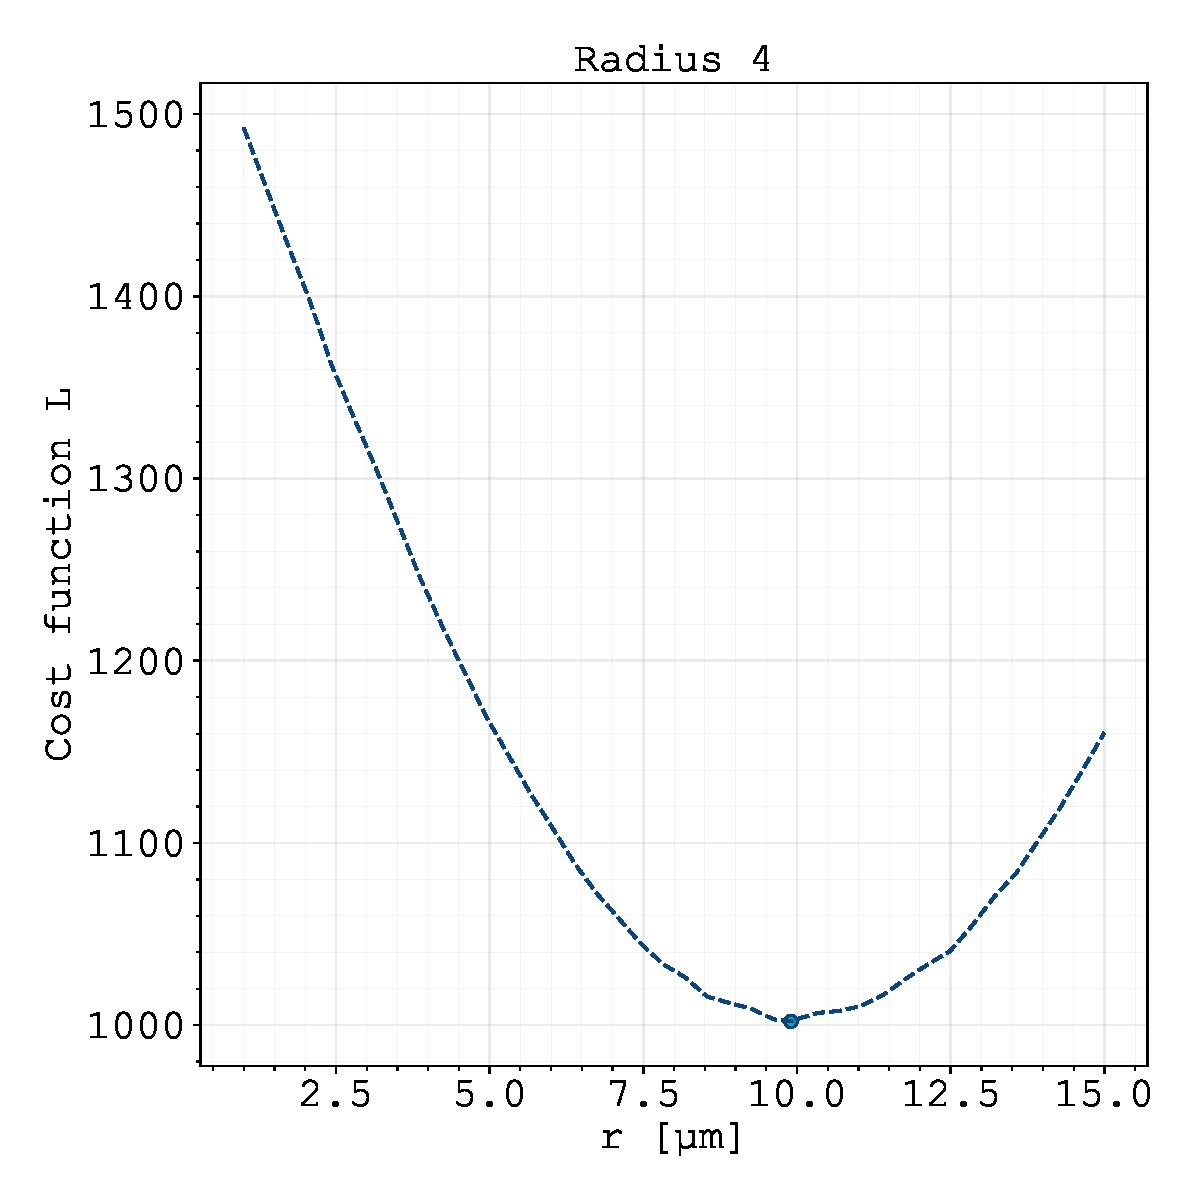
\includegraphics[width=0.33\textwidth]
        {figures/crm_fit/profiles/radius-4.pdf}%
    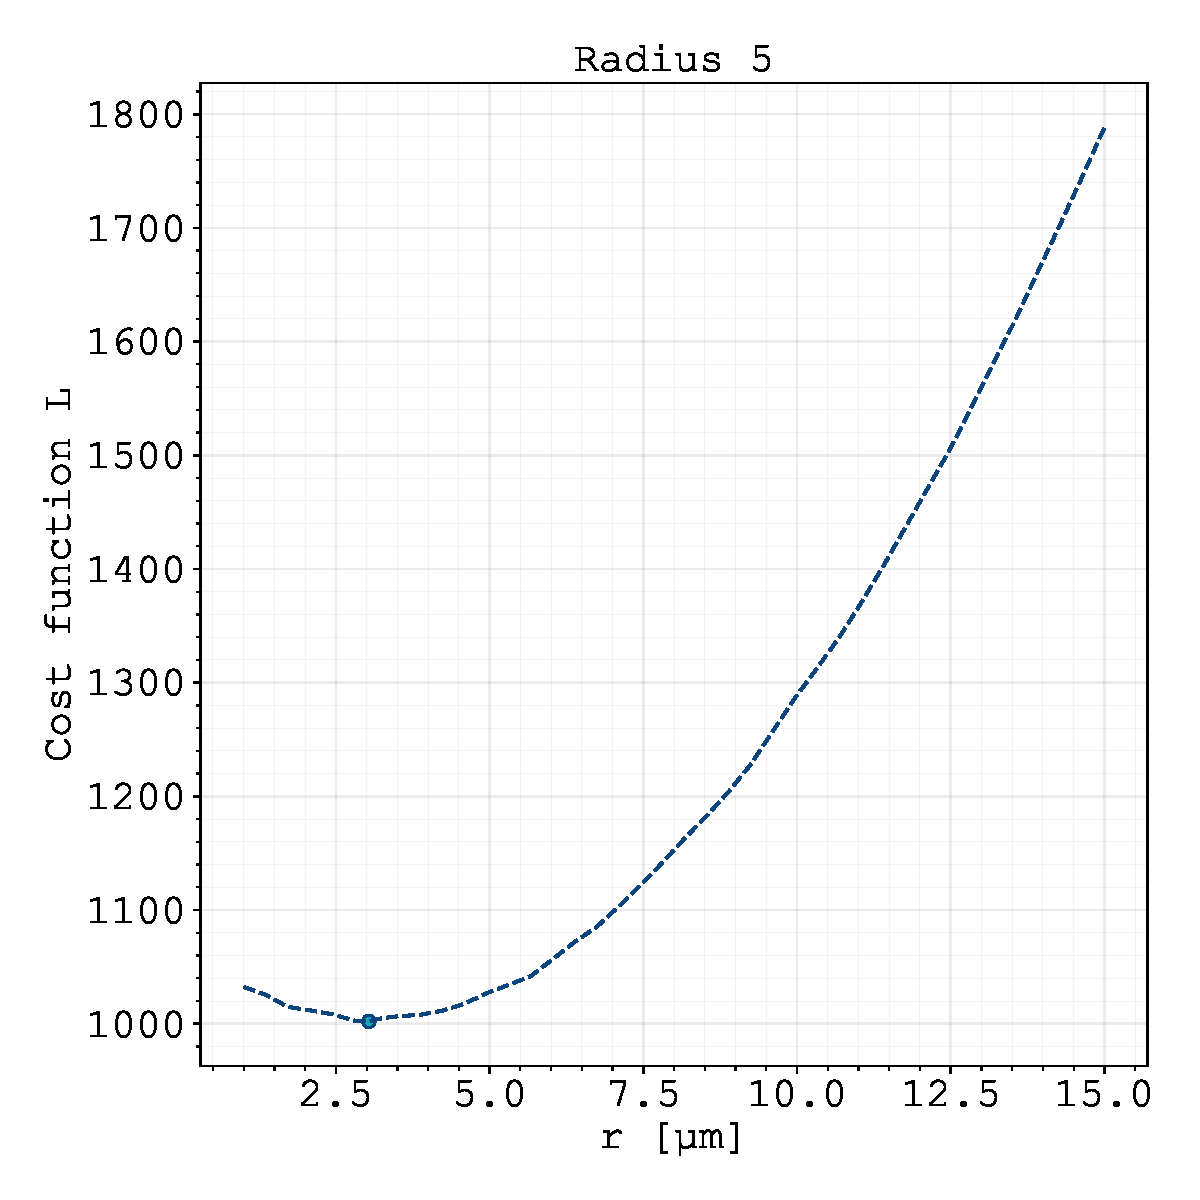
\includegraphics[width=0.33\textwidth]
        {figures/crm_fit/profiles/radius-5.pdf}%
    \caption{Parameter estimation of radii for individual cells}%TODO extend caption}
    \label{fig:parameter-estimates-supplement-radii}
\end{figure}

%###################################################################################################
\section{More Simulation Aspects}
\label{section:supplement-more-simulation-aspects}
%TODO insert this into the discussion later
\begin{table}[H]
    \centering
    \def\arraystretch{1.3}
    \begin{tabularx}{\textwidth}{c l X}
        &\textbf{Aspect} & \textbf{Description}\\
        \toprule
        &\textbf{(C) Cellular}\\
        \midrule
        (1) & Rod-Shaped Mechanics &
            Rod-shaped bacteria are flexible rods which are able to freely move around (off-lattice
            approach) \cite{Takeuchi2005,Ursell2014,Amir2014_2}.\\
        (2) & Growth &
            Cells grow exponentially by inserting new material along the circular part of the rod
            \cite{Robert2014,Takeuchi2005}.\\
        (3) & Differentiation &
            \textit{B.subtilis} is known to differentiate into matrix-producing and
            surfactin-producing cells \cite{vanGestel2015,Lpez2010}.\\
        (4) & Division &
            The formation and continuation of van Gogh bundles is driven by cell division
            \cite{vanGestel2015}.
            Bacteria can form multilayers during their growth phase \cite{Duvernoy2018}.\\
        (5) & Variable Parameters &
            Parameters for individual cells are not fixed values but rather taken from a
            distribution \cite{Koutsoumanis2013}.\\
        &\textbf{(CC) Cell-Cell Interactions}\\
        \midrule
        (6) & Adhesion &
            Bacteria adhere to each other at longer distances and attach when in close contact
            \cite{Verwey1947,Trejo2013}.
            The interaction between rods can be polarized \cite{Duvernoy2018}.\\
        (7) & Friction &
            Friction between cells \cite{Grant2014} can be asymmetrical \cite{Doumic2020}.\\
        &\textbf{(DC) Domain-Cell Interactions}\\
        \midrule
        (8) & External Forces &
            Bacteria tend to stick to surfaces \cite{vanLoosdrecht1989}.
            The extracellular gel exerts a force onto the cells \cite{Grant2014}.\\
        (9) & Extracellular Reactions &
            Bacteria can take up nutrients or possible secrete/take up signalling molecules
            \cite{Li2025}.\\
        \bottomrule
    \end{tabularx}
    \label{table:simulation-aspects-supplement}
    \caption{TODO Insert caption}
\end{table}

%###################################################################################################
\section{Performance}

\begin{itemize}
    \item Quadratic Scaling comes from more dense simulation
    \item Overall number of agents which can be simulated is satisfactory for current purposes
    \item Improvement from $1 \Rightarrow 2$ and $2\Rightarrow4$ threads; first is major; second
        only minor
    \item Flamegraph still shows much cycles running against hurdles::Barrier::wait $\Rightarrow$
        this leaves room for improvement
    \item Flamegraph also shows that $\approx 75\%$ of all cycles is related to actual work (not
        just waiting).
        In particular to update\_mechanics functions.
\end{itemize}

\begin{figure}[H]
    \centering
    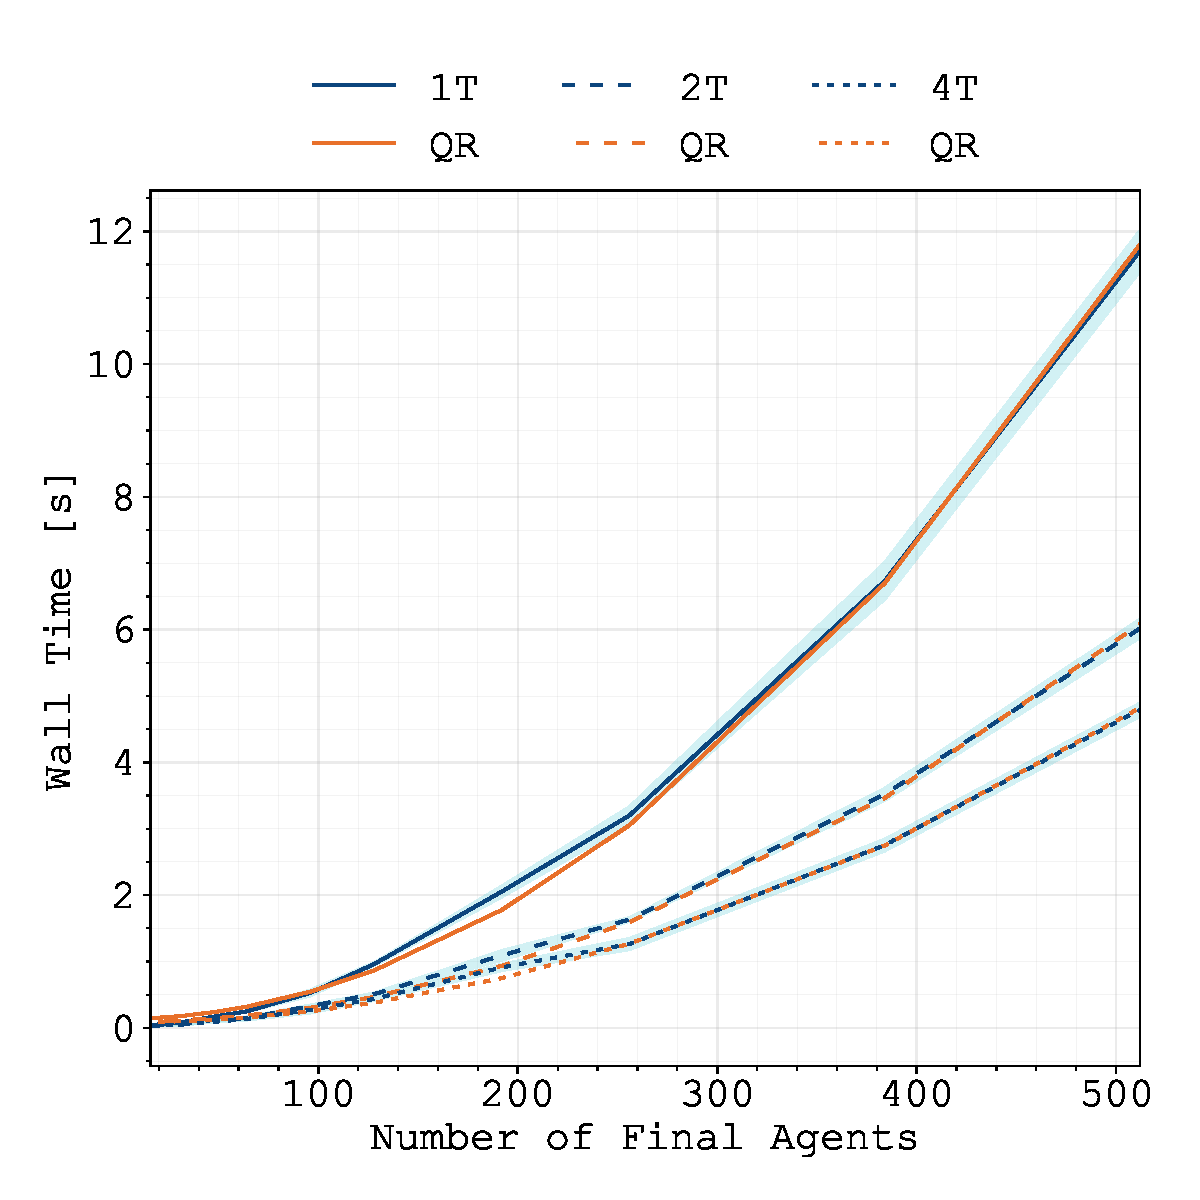
\includegraphics[width=0.49\textwidth]
        {docs/source/_static/performance/computation-time-with-initial-agents.pdf}
    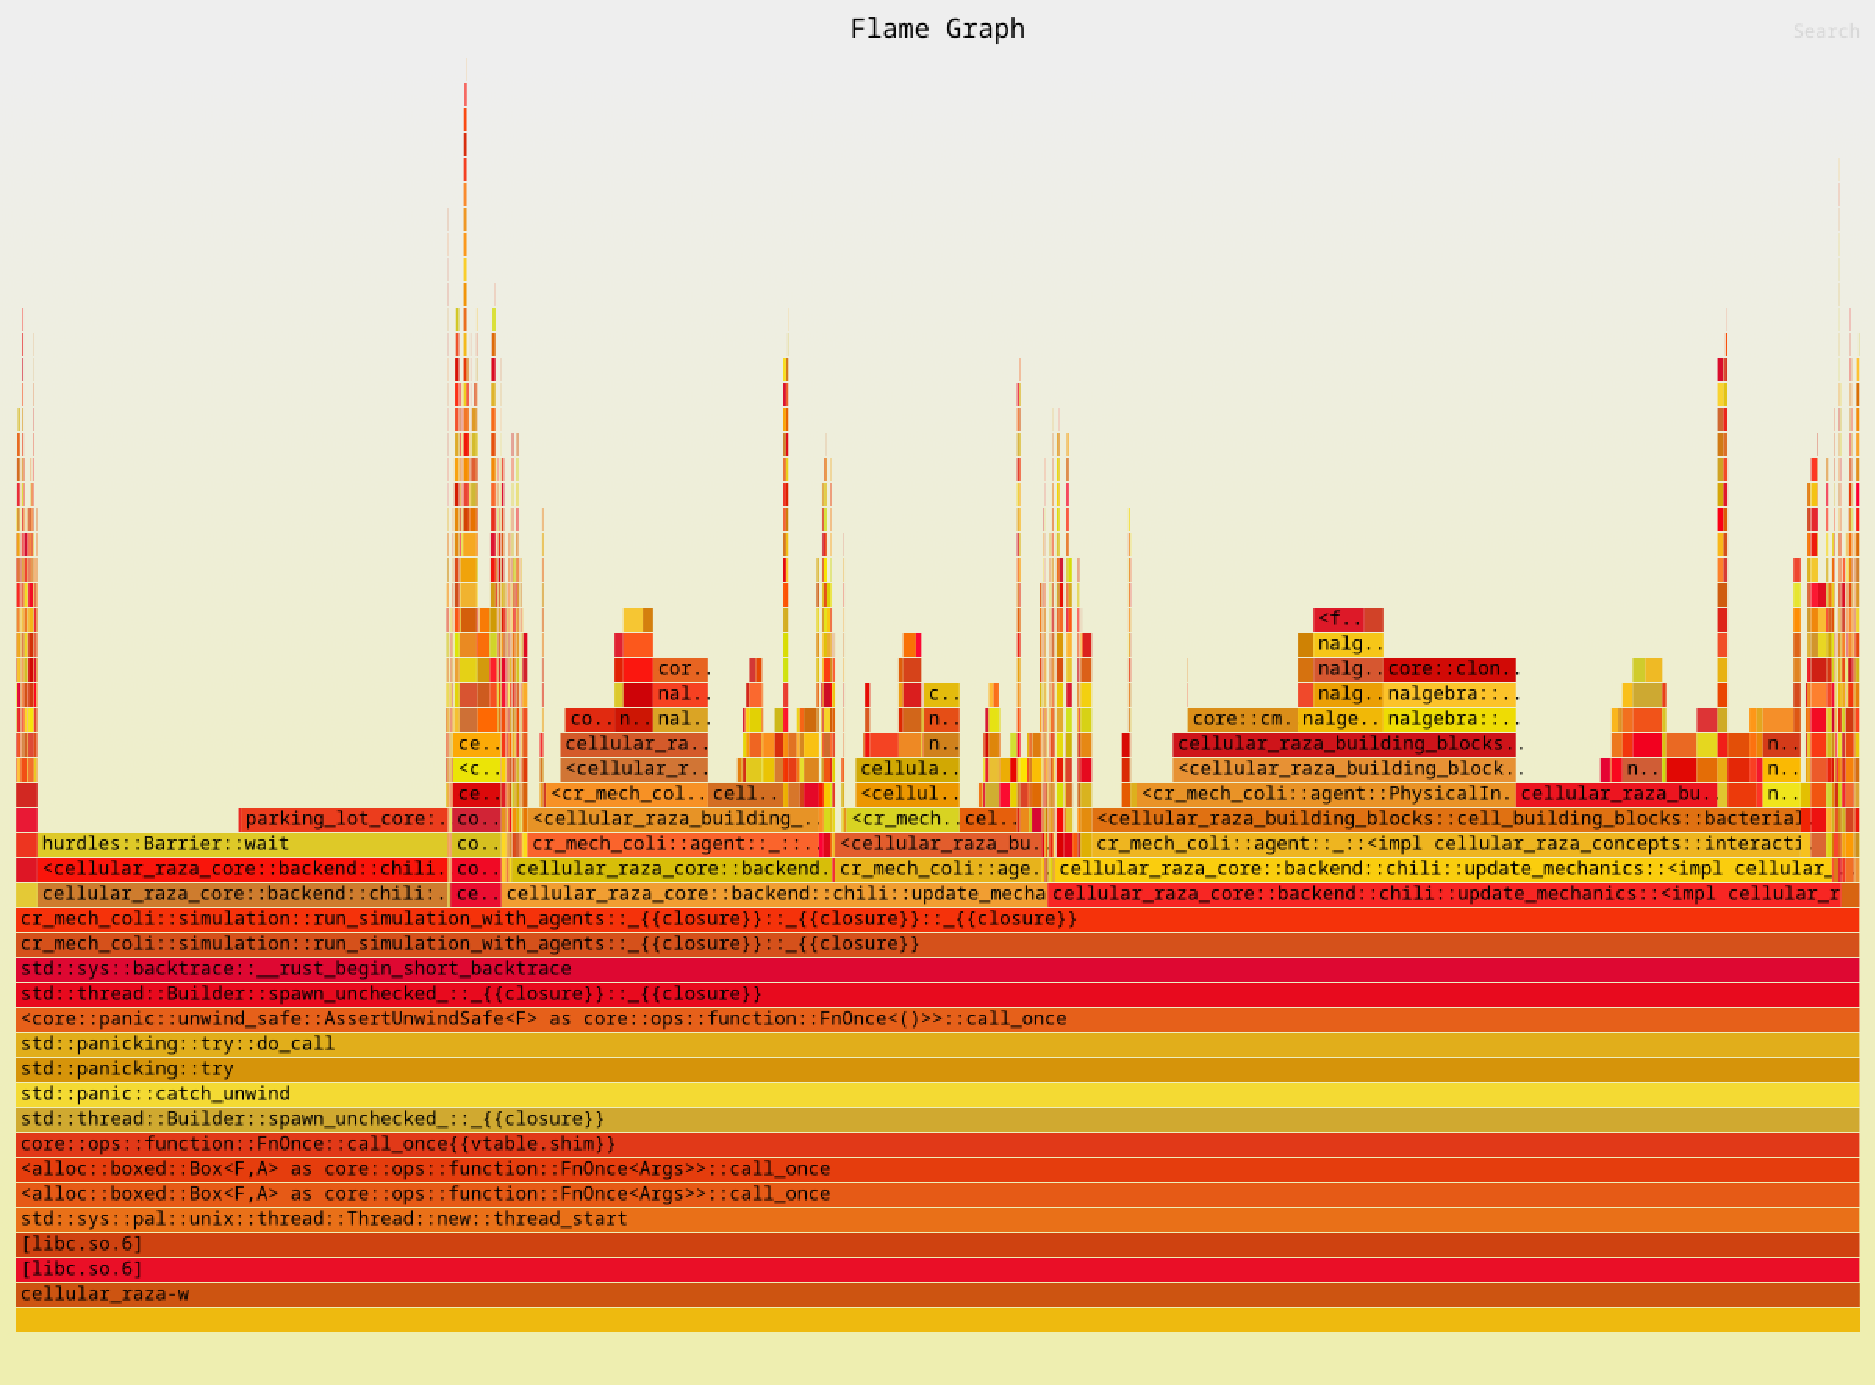
\includegraphics[width=0.49\textwidth]{docs/source/_static/performance/flamegraph.pdf}
    \caption{TODO}
    \label{fig:performance}
\end{figure}

%###################################################################################################
\section{Multilayer Predictions}
% TODO
\begin{itemize}
    \item Do we need this in this publication?
    \item Maybe this is out of scope as this is a more methodological paper.
    \item If we want to omit it, we might also opt to change the model description in the beginning
        and remove some parts of the external forces discussion.
\end{itemize}

\begin{figure}[H]
    \centering
    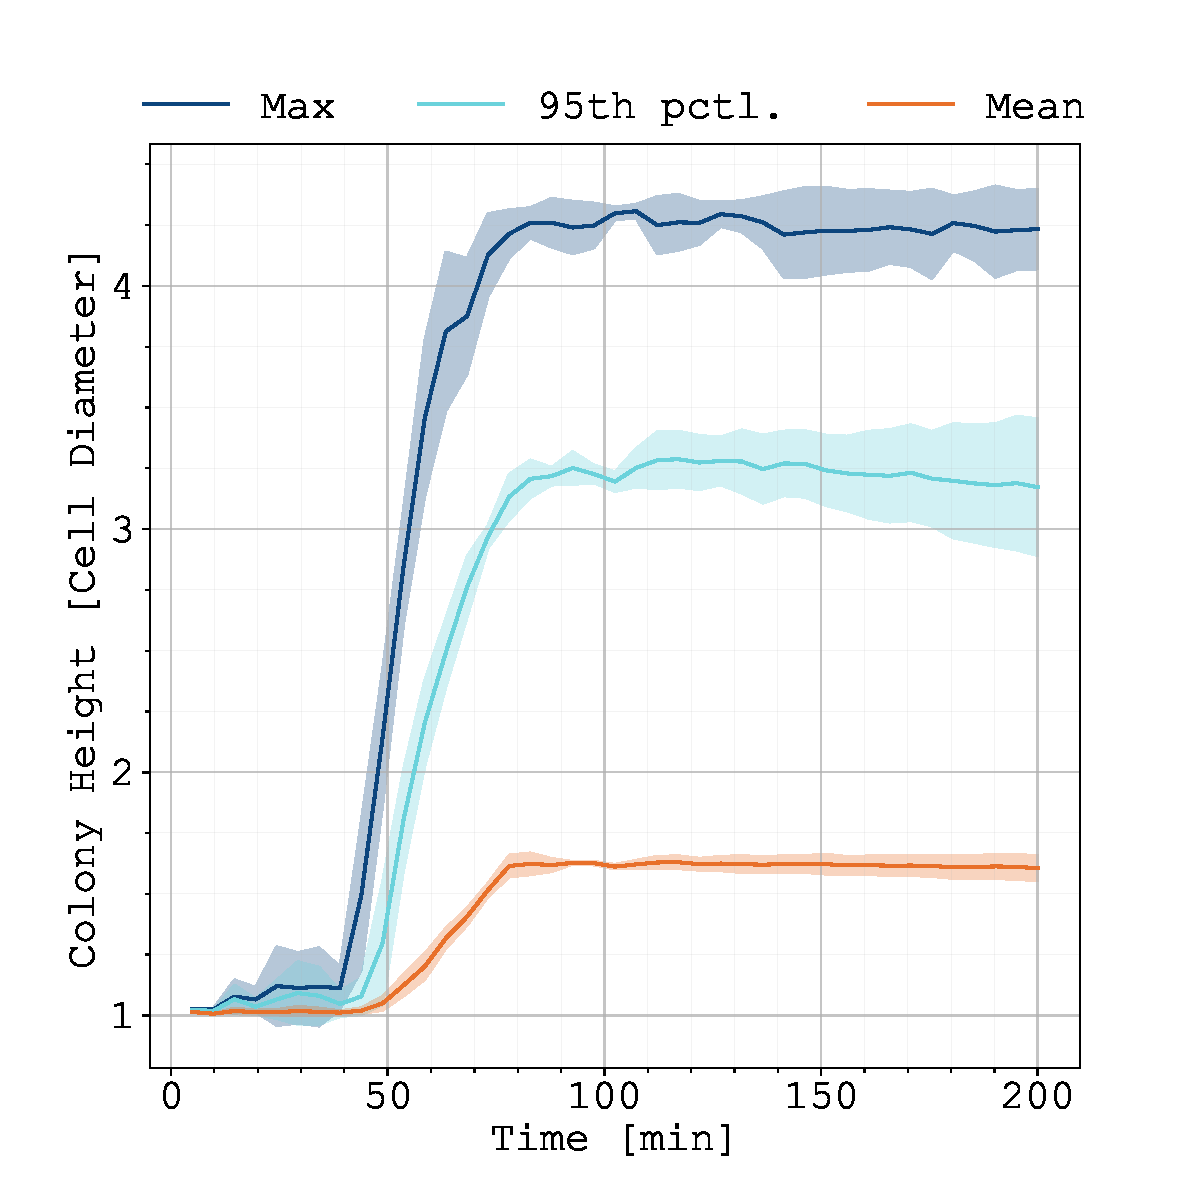
\includegraphics[width=0.49\textwidth]
        {docs/source/_static/scripts/crm_multilayer/multilayer-time-evolution.pdf}\\
    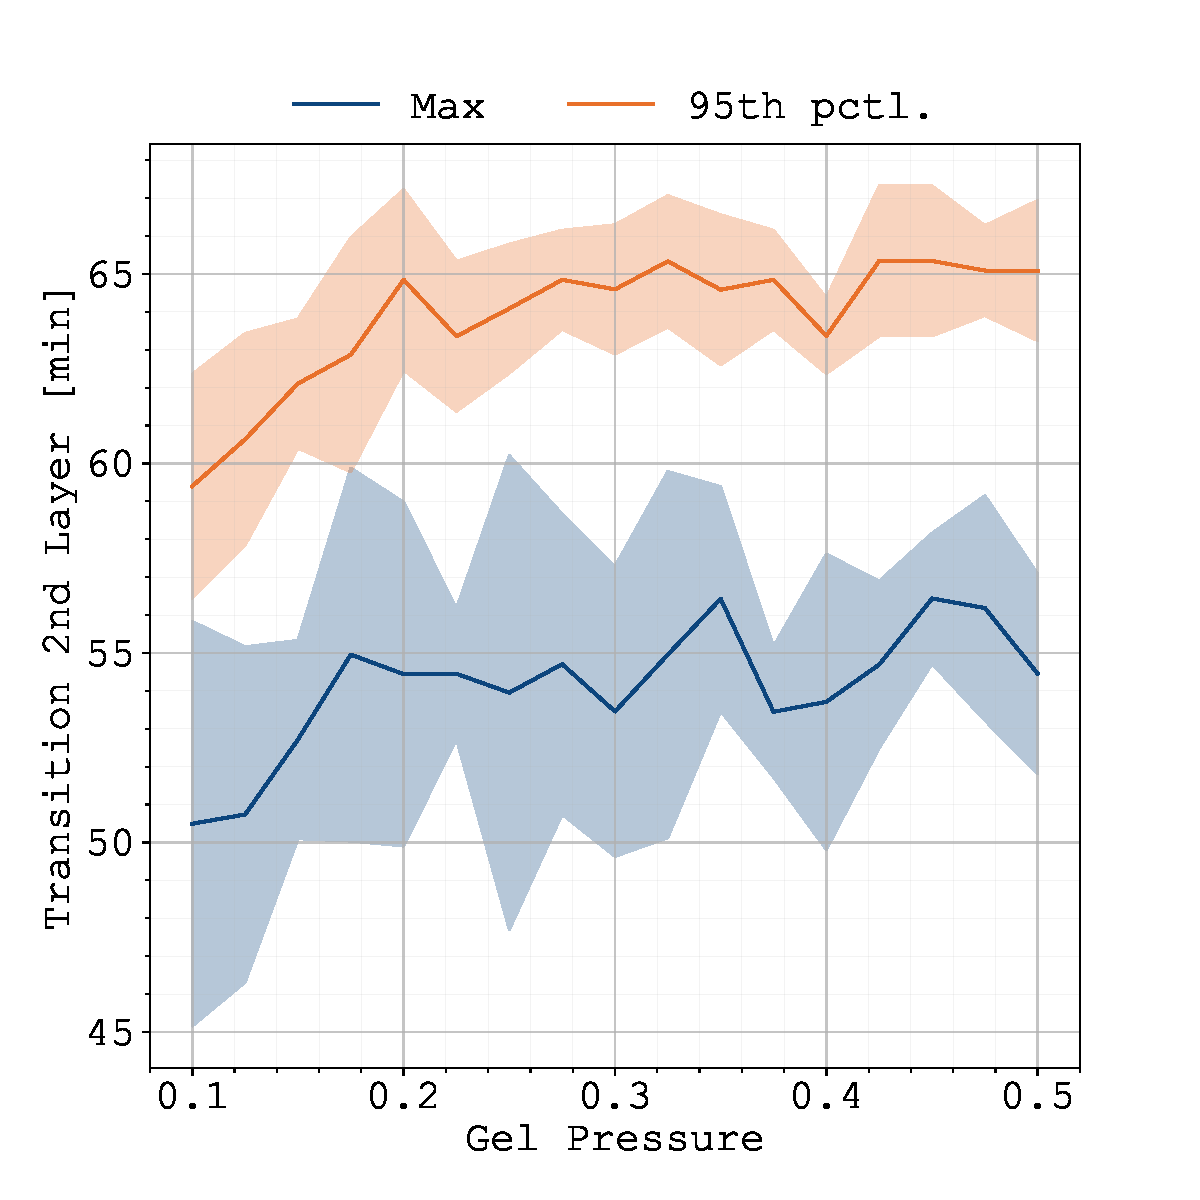
\includegraphics[width=0.49\textwidth]
        {docs/source/_static/scripts/crm_multilayer/colony-height-vs-gel_pressure.pdf}
    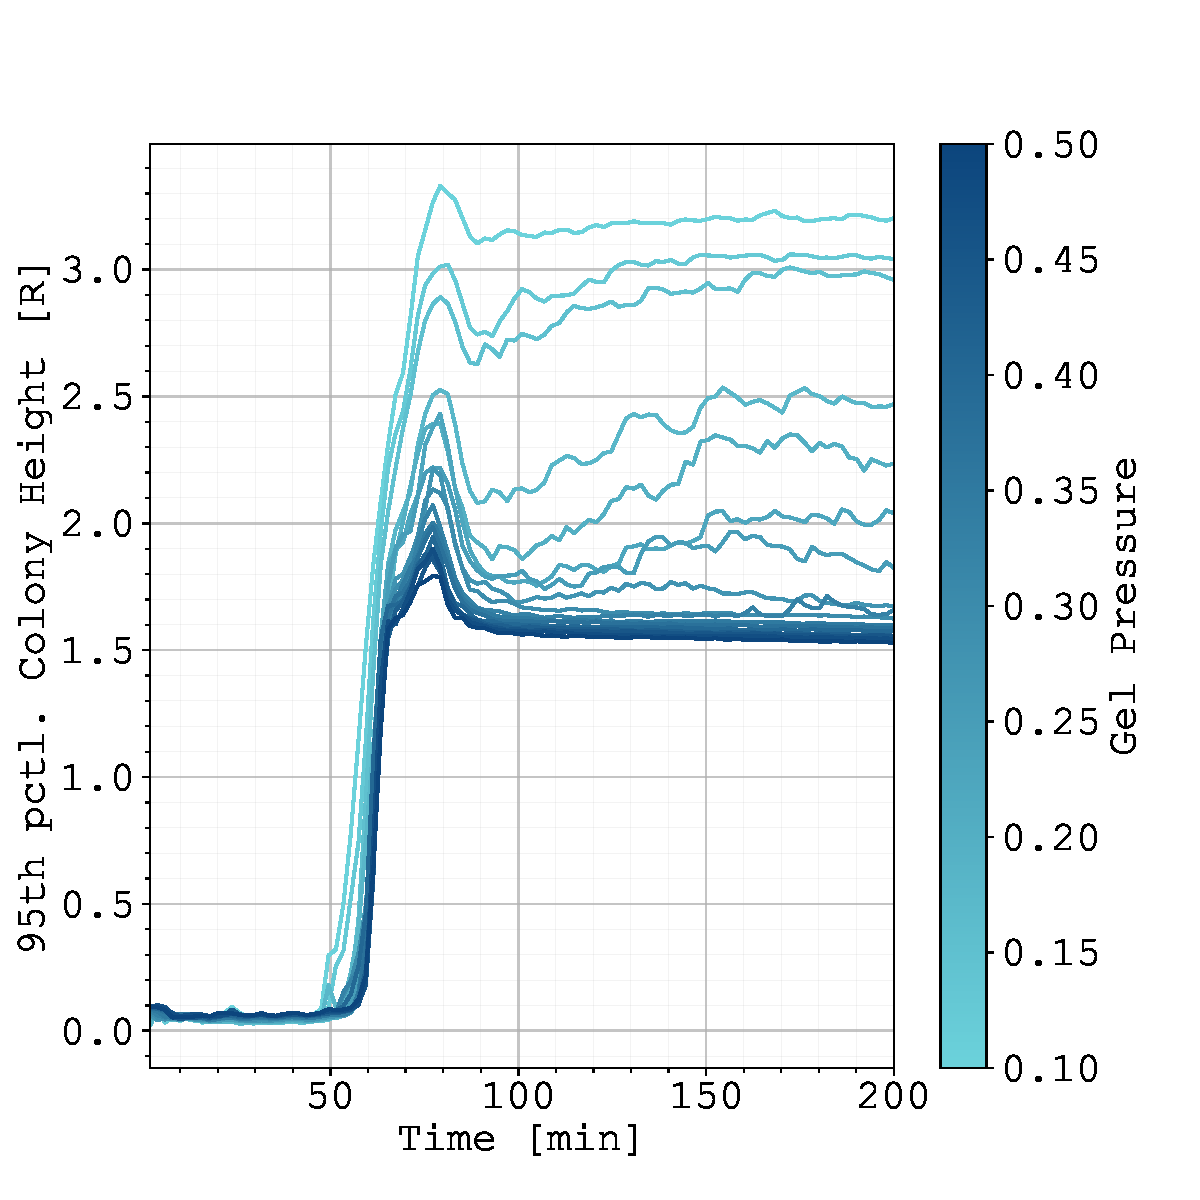
\includegraphics[width=0.49\textwidth]
        {docs/source/_static/scripts/crm_multilayer/colony-height-vs-time.pdf}
    \caption{TODO}
    \label{fig:multilayer}
\end{figure}


\end{document}
